% !TeX root = d2.tex

\documentclass{article}

% \usepackage{xcolor}
\usepackage[margin=0.5in]{geometry} 
\usepackage{graphicx}
\usepackage{multirow}
\usepackage[table,xcdraw]{xcolor}
\usepackage[normalem]{ulem}
\usepackage{float}
\usepackage{adjustbox, lipsum}
\usepackage{pdfpages}
\useunder{\uline}{\ul}{}
\title{MindMerge --- Deliverable e 2}
\author{Gabriele Benetti, Gioele Bernardini, Luca Fossa Crescini, Luca Sartore}

\begin{document}
\maketitle


\tableofcontents


\newpage
\section*{Abstract}   % titolo temporaneo da modificare
This is the Abstract of the deliverable 2

\section{Architecture description}


\begin{figure}[h]
  \centering
  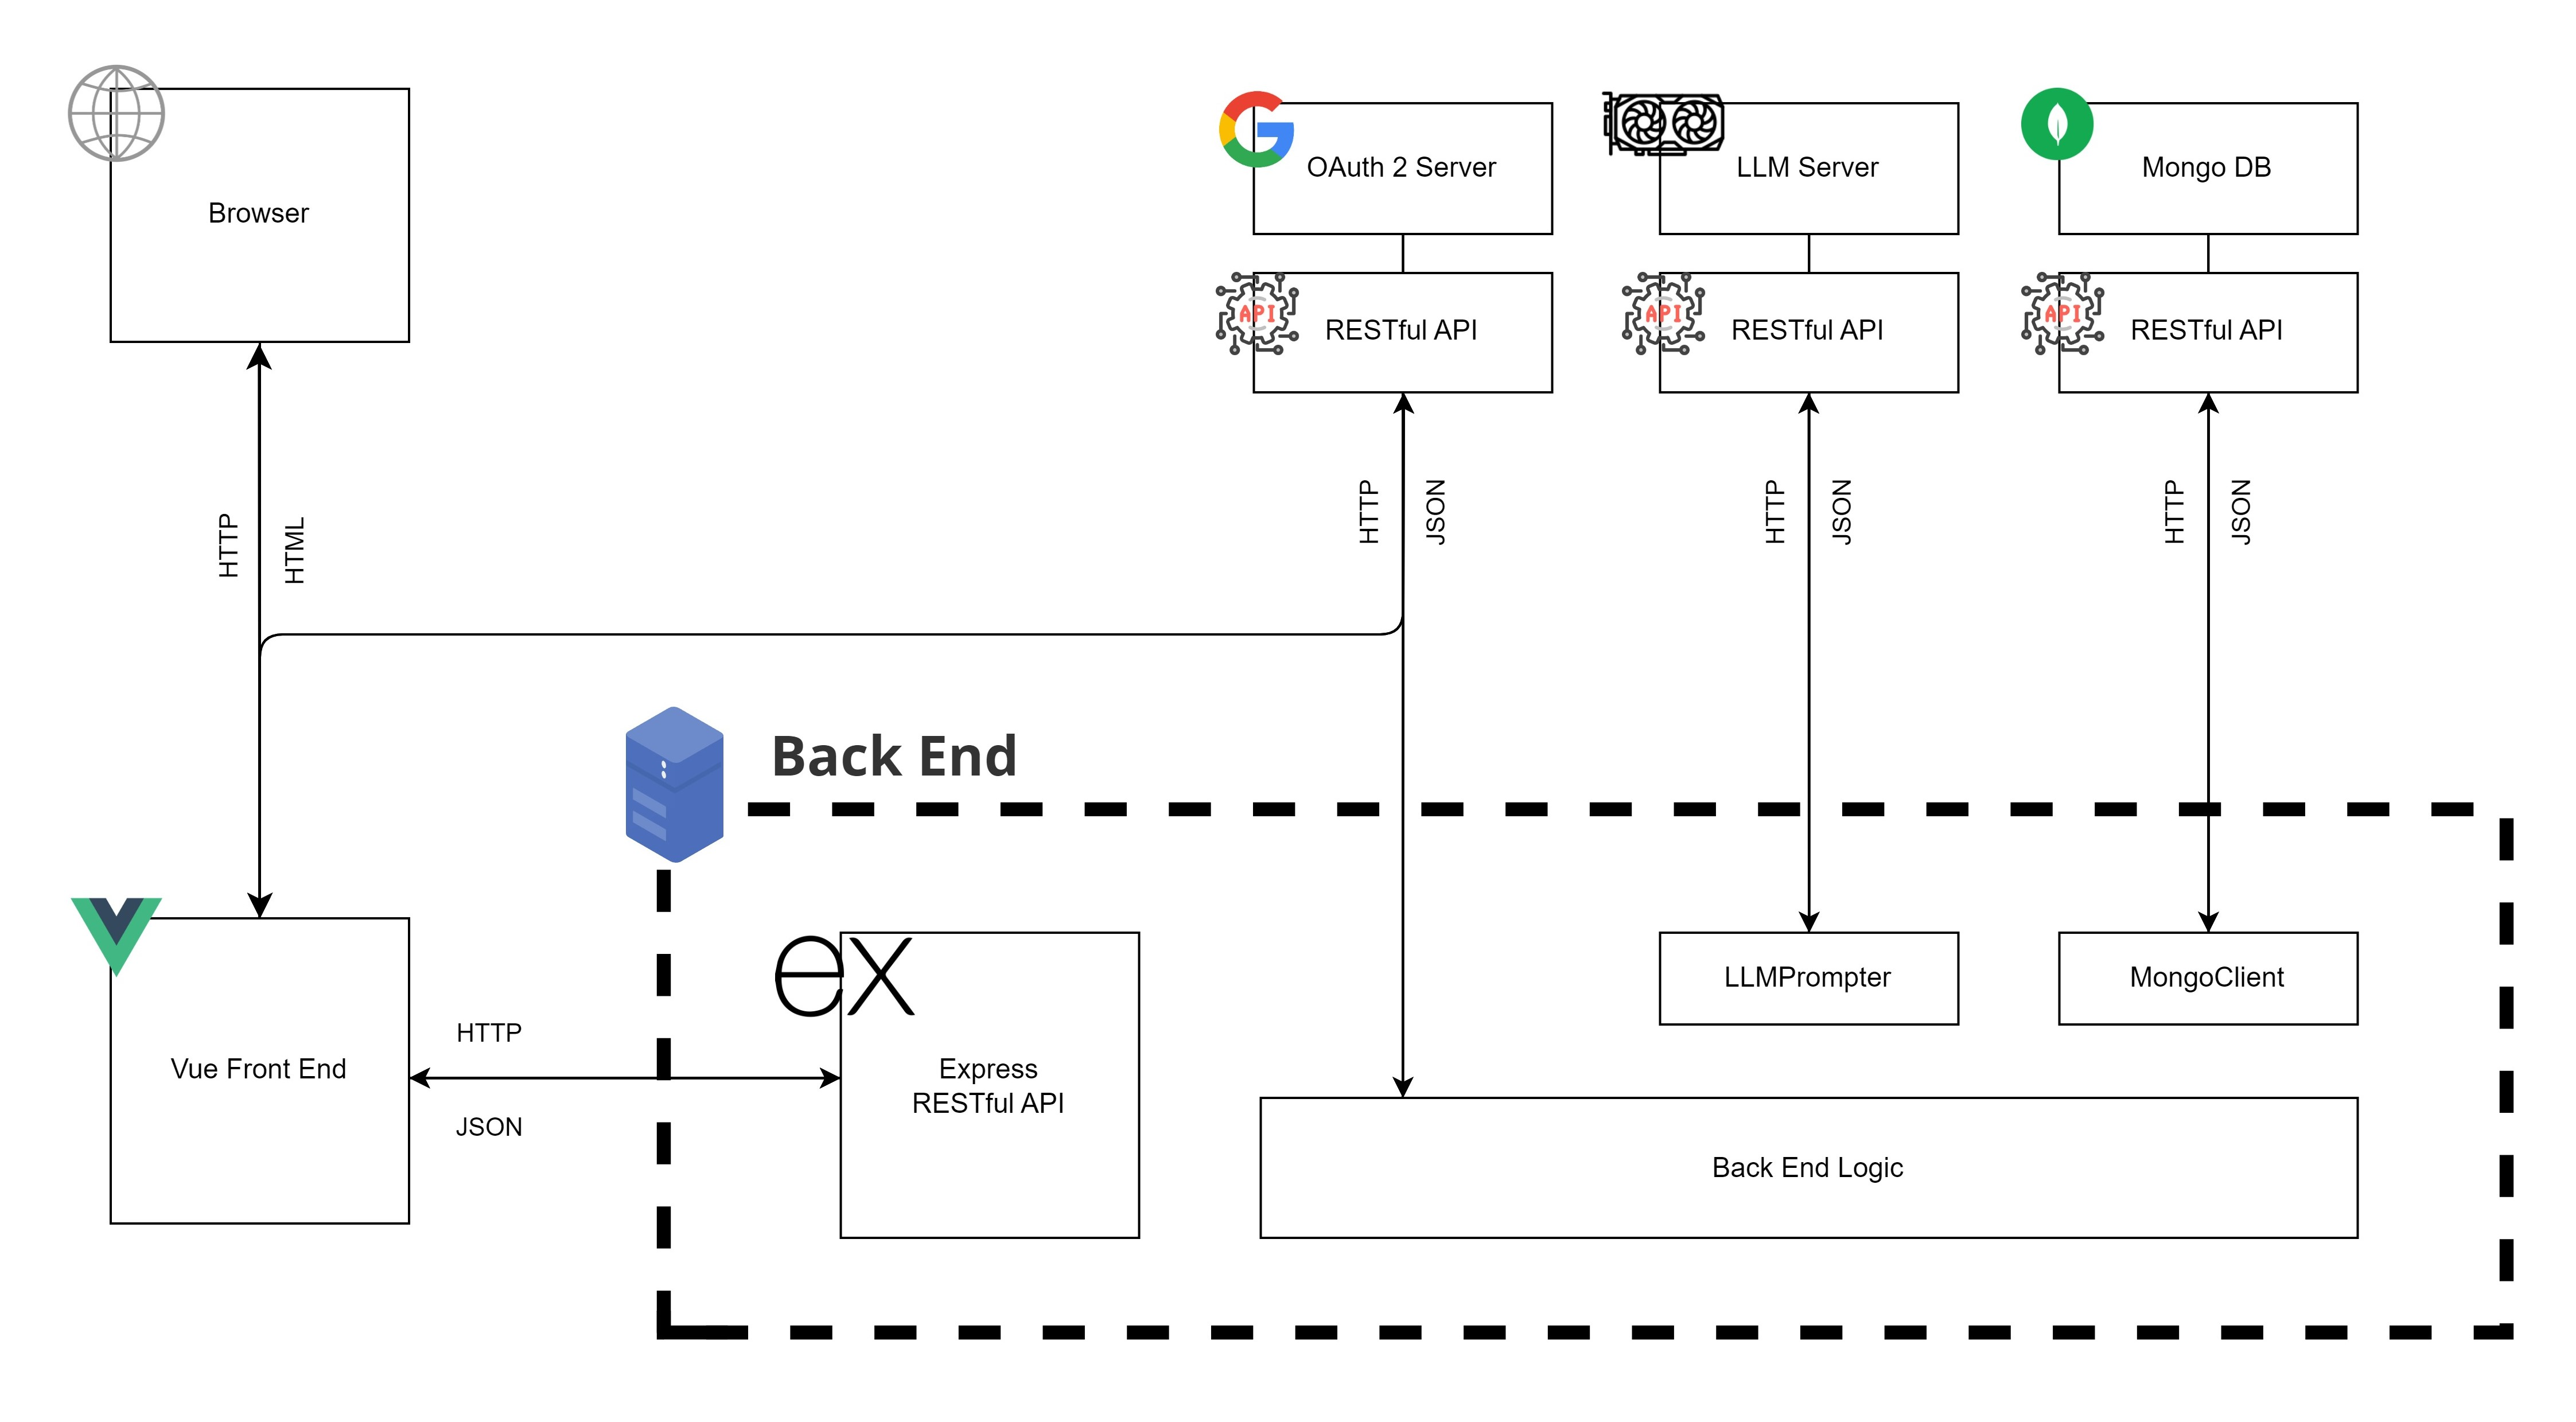
\includegraphics[width=0.95\textwidth]{images/architecture.jpg}
  \caption{\small The architecture diagram ot the MindMerge system}
\end{figure}
The architecture is relatively simple,
comprising two classical components: the front end and the back end, along with several smaller components (browser, OAuth server, LLM service, and MongoDB).
\newline \newline
The browser communicates with the front end using the HTTP protocol and HTML format.
\newline \newline
The front end, based on the Vue library, accesses resources provided by the back end using HTTP with JSON data format.
\newline \newline
Authentication is provided by a third-party OAuth server, that communicate with both the front end and back end via HTTP/JSON.
\newline \newline
The back end is the most complex component consists of several sub-components, including:
\begin{itemize}
  \item A part providing RESTful APIs based on Express.js
  \item A component dedicated to communicating with the database (MongoClient)
  \item A module for communicating with the LLM service (LLMPrompter)
  \item Logic containing all functions necessary for the application's operation.
\end{itemize}
All the communications that the backend has with the external world are made through HTTP with json format.

\section{Product Backlog}


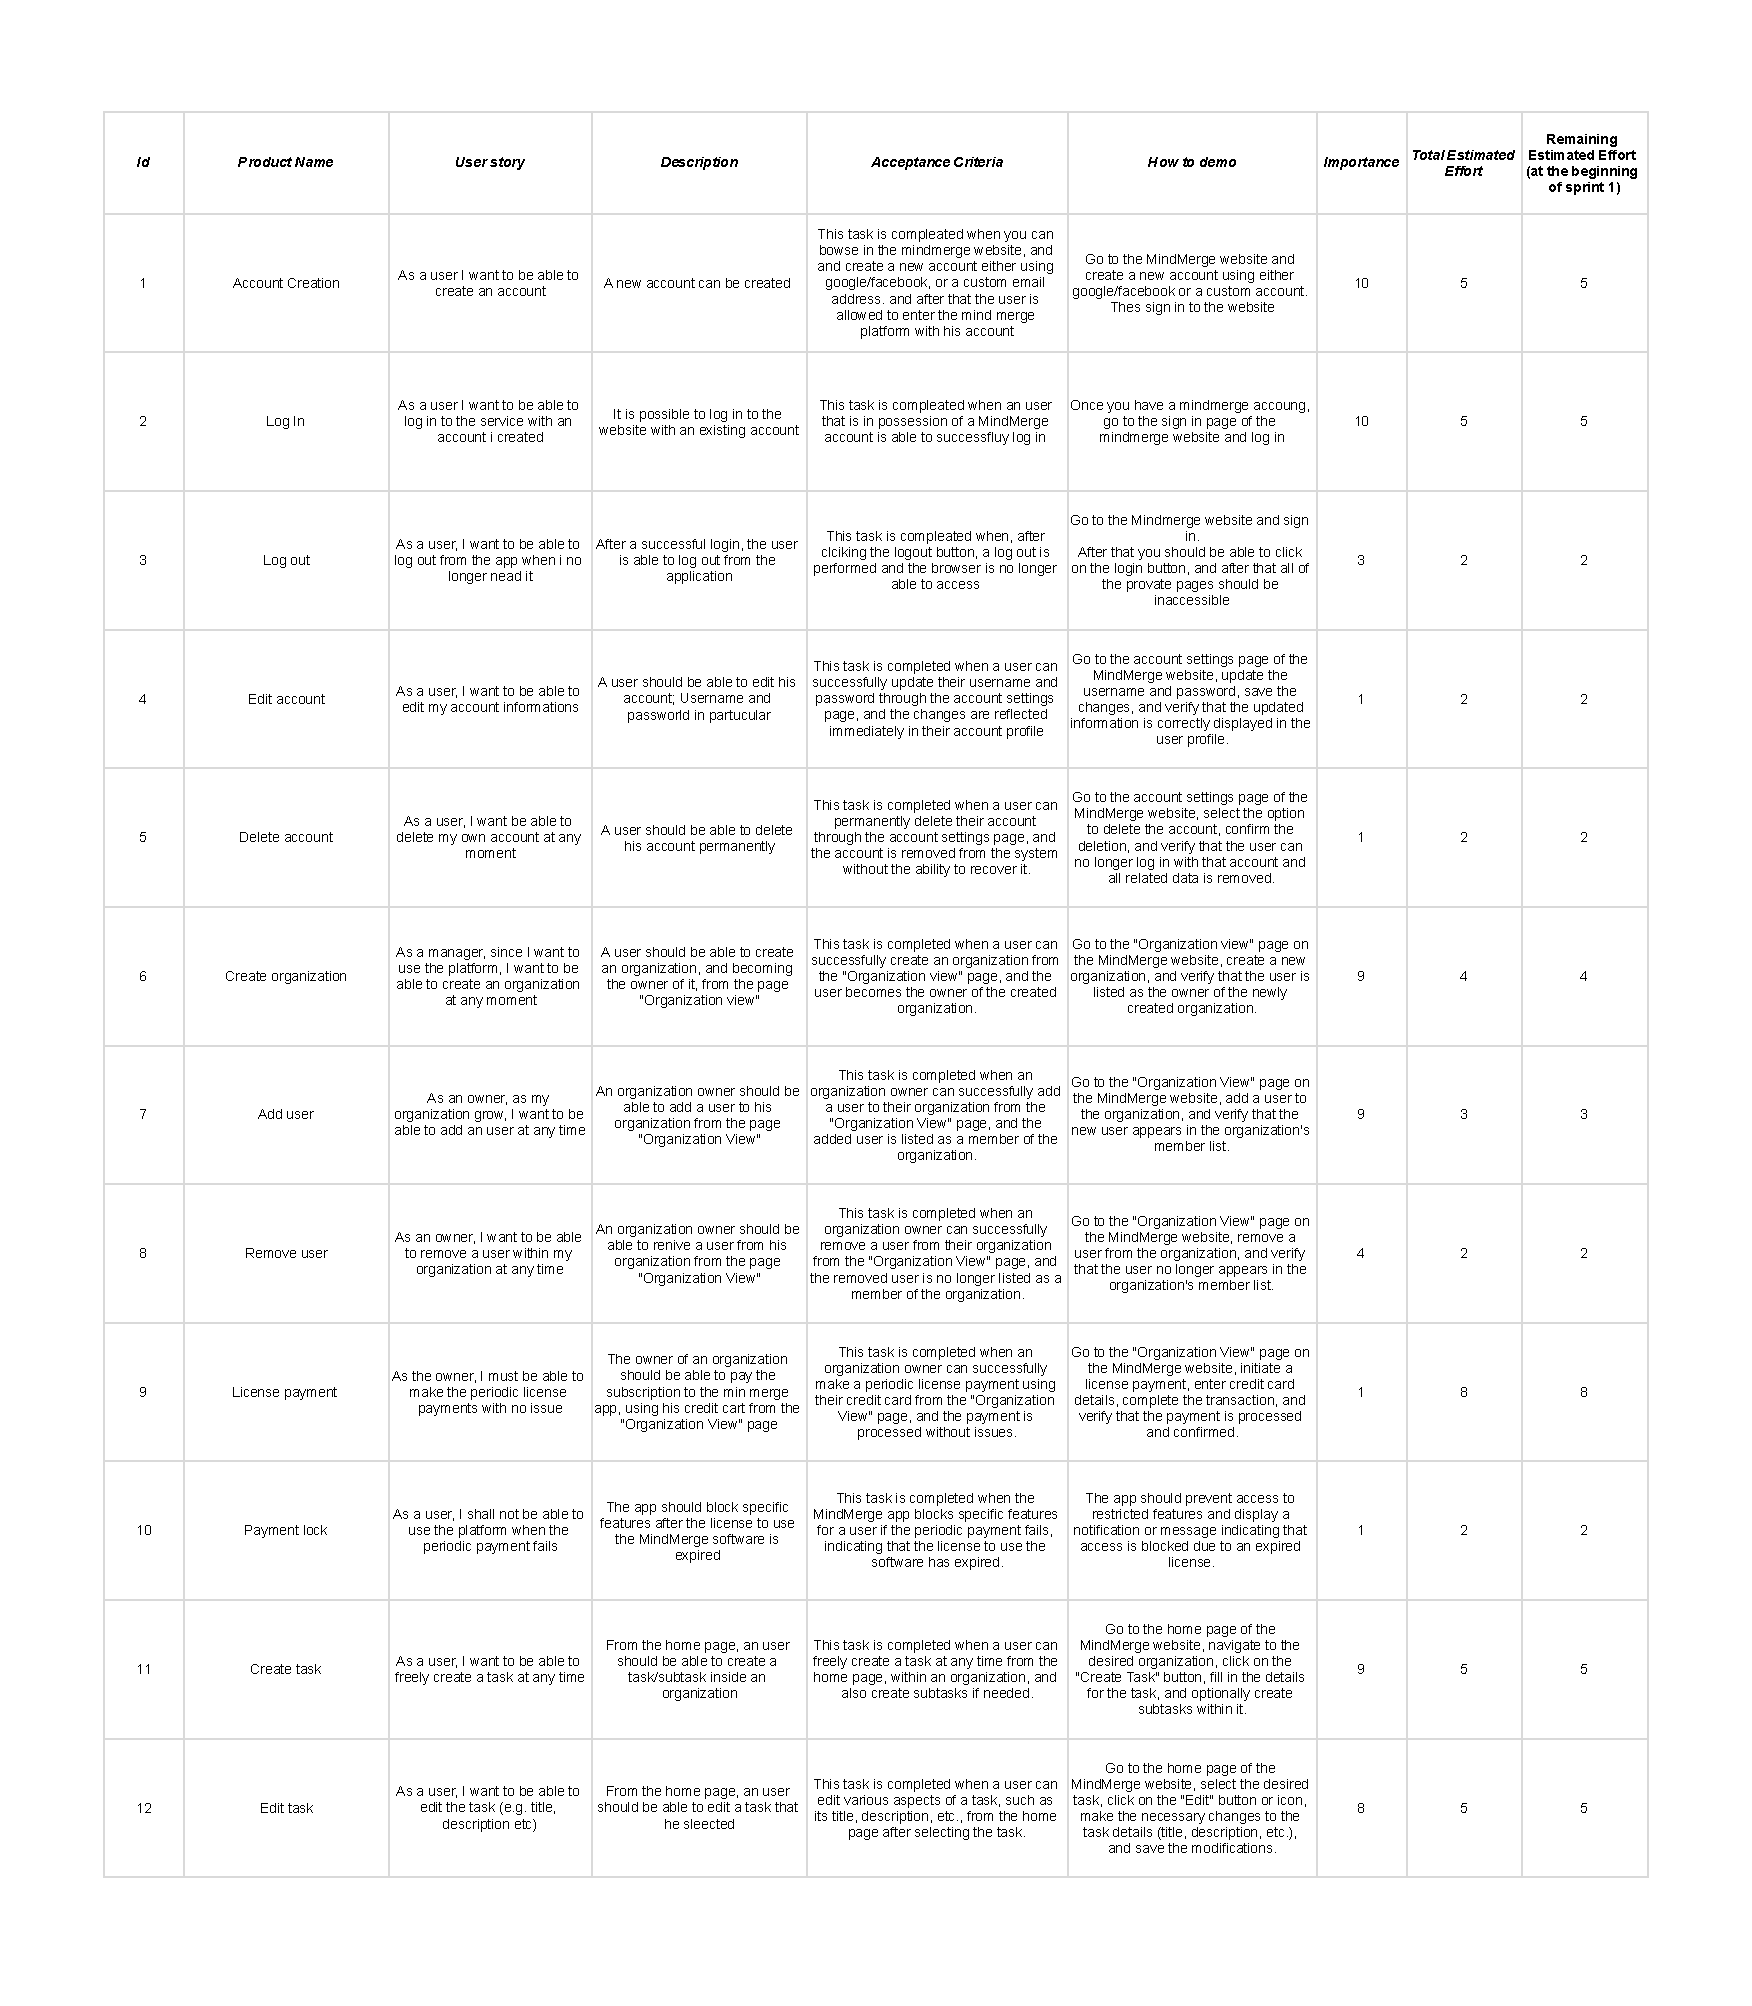
\includepdf[pages=-]{images/product_backlog.pdf}

\section{Definition of Tests}

\subsection*{Test DatabaseManager:TaskManager}

This section contains the tests for the TaskManager class, which is responsible for managing tasks in the database.
\newline
\adjustbox{max width=\textwidth}{
  \begin{tabular}{|l|c|l|l|l|l|l|}
    \hline
    \multicolumn{1}{|c|}{\cellcolor[HTML]{FFFFFF}\textbf{Number}} & \cellcolor[HTML]{FFFFFF}\textbf{Test Group}                                  & \multicolumn{1}{c|}{\cellcolor[HTML]{FFFFFF}\textbf{Test Type}} & \multicolumn{1}{c|}{\textbf{Name}}             & \multicolumn{1}{c|}{\textbf{Test case data}}                                                                                     & \multicolumn{1}{c|}{\textbf{Preconditions}}                                                    & \multicolumn{1}{c|}{\textbf{Expected Results}}                                                                                \\ \hline
    \rowcolor[HTML]{FFFFFF}
    1                                                             & \cellcolor[HTML]{FFFFFF}                                                     & {\color[HTML]{11734B} Automated}                                & successul task creation                        & Call the method TaskManager.createTask three times with different task names and check the results.                              & The TaskModel collection is empty.                                                             & A new task is created each time with the expected attributes and status code. The tasks are correctly stored in the database. \\ \cline{1-1} \cline{3-7}
    \rowcolor[HTML]{FFFFFF}
    2                                                             & \cellcolor[HTML]{FFFFFF}                                                     & {\color[HTML]{11734B} Automated}                                & unsuccessul task creation                      & Call the method TaskManager.createTask with various invalid task data                                                            & The TaskModel collection is empty.                                                             & Errors.BAD\_REQUEST is returned                                                                                               \\ \cline{1-1} \cline{3-7}
    \rowcolor[HTML]{FFFFFF}
    3                                                             & \cellcolor[HTML]{FFFFFF}                                                     & {\color[HTML]{11734B} Automated}                                & successul task note creation                   & Call the method TaskManager.createTaskNotes and pass a valid taskId and notes                                                    & The TaskModel has a few tasks created where notes can be added                                 & Notes for tasks are created                                                                                                   \\ \cline{1-1} \cline{3-7}
    \rowcolor[HTML]{FFFFFF}
    4                                                             & \cellcolor[HTML]{FFFFFF}                                                     & {\color[HTML]{11734B} Automated}                                & unsuccessul task note creation                 & Call the method TaskManager.createTaskNotes with invalid parameters, and/or with non existing task                               & The TaskModel has a few tasks created where notes can be added                                 & Errors.NOT\_FOUND or Errors.BAD\_REQUEST is returned based on the invalid parameters                                          \\ \cline{1-1} \cline{3-7}
    \rowcolor[HTML]{FFFFFF}
    5                                                             & \cellcolor[HTML]{FFFFFF}                                                     & {\color[HTML]{11734B} Automated}                                & successful task report schedule creation       & Call TaskManager.createTaskReportSchedule with valid report schedule data                                                        & The TaskModel has a few tasks created where schedules can be added                             & A successful status code is returned and the task report schedules are created correctly.                                     \\ \cline{1-1} \cline{3-7}
    \rowcolor[HTML]{FFFFFF}
    6                                                             & \cellcolor[HTML]{FFFFFF}                                                     & {\color[HTML]{11734B} Automated}                                & unsuccessful task report schedule creation     & Call TaskManager.createTaskReportSchedule with invalid report schedule data                                                      & The TaskModel has a few tasks created where schedules can be added                             & Errors.NOT\_FOUND or Errors.BAD\_REQUEST is returned based on the invalid parameters                                          \\ \cline{1-1} \cline{3-7}
    \rowcolor[HTML]{FFFFFF}
    7                                                             & \cellcolor[HTML]{FFFFFF}                                                     & {\color[HTML]{11734B} Automated}                                & successful task update                         & Call the method TaskManager.updateTask and pass valid parameters                                                                 & The TaskModel has a few tasks created that can be edited for the test                          & Tasks are successfully updated with the correct data                                                                          \\ \cline{1-1} \cline{3-7}
    \rowcolor[HTML]{FFFFFF}
    8                                                             & \cellcolor[HTML]{FFFFFF}                                                     & {\color[HTML]{11734B} Automated}                                & unsuccessful task update                       & Call the method TaskManager.updateTask and pass non valid parameters                                                             & The TaskModel has a few tasks created that can be edited for the test                          & Errors.NOT\_FOUND or Errors.BAD\_REQUEST is returned based on the invalid parameters                                          \\ \cline{1-1} \cline{3-7}
    \rowcolor[HTML]{FFFFFF}
    9                                                             & \cellcolor[HTML]{FFFFFF}                                                     & {\color[HTML]{11734B} Automated}                                & successful update last task update             & Call TaskManager.updateTaskLastUpdated and pass the id of an existing task                                                       & The TaskModel has a few tasks created that can be edited for the test                          & The task's lastUpdated field is updated correctly, with the current time                                                      \\ \cline{1-1} \cline{3-7}
    \rowcolor[HTML]{FFFFFF}
    10                                                            & \cellcolor[HTML]{FFFFFF}                                                     & {\color[HTML]{11734B} Automated}                                & unsuccessful update last task update           & Call TaskManager.updateTaskLastUpdated and pass the id of a non existing task                                                    & The TaskModel has a few tasks created that can be edited for the test                          & The expected status code for each update attempt is Errors.NOT\_FOUND                                                         \\ \cline{1-1} \cline{3-7}
    \rowcolor[HTML]{FFFFFF}
    11                                                            & \cellcolor[HTML]{FFFFFF}                                                     & {\color[HTML]{11734B} Automated}                                & successful update task name                    & Call the method TaskManager.updateTaskName with valid task and organization IDs, and a new task name                             & The TaskModel has a few tasks created that can be edited for the test                          & The task's name is successfuly updated in the database                                                                        \\ \cline{1-1} \cline{3-7}
    \rowcolor[HTML]{FFFFFF}
    12                                                            & \cellcolor[HTML]{FFFFFF}                                                     & {\color[HTML]{11734B} Automated}                                & unsuccessful update task name                  & Call the method TaskManager.updateTaskName with invalid task and organization IDs, and/or an invalid name                        & The TaskModel has a few tasks created that can be edited for the test                          & Errors.NOT\_FOUND or Errors.BAD\_REQUEST is returned based on the invalid parameters                                          \\ \cline{1-1} \cline{3-7}
    \rowcolor[HTML]{FFFFFF}
    13                                                            & \cellcolor[HTML]{FFFFFF}                                                     & {\color[HTML]{11734B} Automated}                                & successful update task description             & Call the method TaskManager.updateTaskDescription with valid task data                                                           & The TaskModel has a few tasks created that can be edited for the test                          & The task's description is successfuly updated in the database                                                                 \\ \cline{1-1} \cline{3-7}
    \rowcolor[HTML]{FFFFFF}
    14                                                            & \cellcolor[HTML]{FFFFFF}                                                     & {\color[HTML]{11734B} Automated}                                & unsuccessful update task description           & Call the method TaskManager.updateTaskDescription with invalid task data                                                         & The TaskModel has a few tasks created that can be edited for the test                          & Errors.NOT\_FOUND or Errors.BAD\_REQUEST is returned based on the invalid parameters                                          \\ \cline{1-1} \cline{3-7}
    \cellcolor[HTML]{FFFFFF}15                                    & \cellcolor[HTML]{FFFFFF}                                                     & \cellcolor[HTML]{FFFFFF}{\color[HTML]{11734B} Automated}        & successful update task status                  & \cellcolor[HTML]{FFFFFF}Call the method TaskManager.updateTaskStatus with valid task and status                                  & \cellcolor[HTML]{FFFFFF}The TaskModel has a few tasks created that can be edited for the test  & \cellcolor[HTML]{FFFFFF}The task's status is successfuly updated in the database                                              \\ \cline{1-1} \cline{3-7}
    \cellcolor[HTML]{FFFFFF}16                                    & \cellcolor[HTML]{FFFFFF}                                                     & \cellcolor[HTML]{FFFFFF}{\color[HTML]{11734B} Automated}        & unsuccessful update task status                & \cellcolor[HTML]{FFFFFF}Call the method TaskManager.updateTaskStatus with invalid task ids and states id                         & \cellcolor[HTML]{FFFFFF}The TaskModel has a few tasks created that can be edited for the test  & \cellcolor[HTML]{FFFFFF}Errors.NOT\_FOUND or Errors.BAD\_REQUEST is returned based on the invalid parameters                  \\ \cline{1-1} \cline{3-7}
    \cellcolor[HTML]{FFFFFF}17                                    & \cellcolor[HTML]{FFFFFF}                                                     & \cellcolor[HTML]{FFFFFF}{\color[HTML]{11734B} Automated}        & successful update task notes                   & \cellcolor[HTML]{FFFFFF}Call the method TaskManager.updateTaskNotes with valid data                                              & \cellcolor[HTML]{FFFFFF}The TaskModel has a few tasks created that can be edited for the test  & \cellcolor[HTML]{FFFFFF}The task's notes are successfuly updated in the database                                              \\ \cline{1-1} \cline{3-7}
    \cellcolor[HTML]{FFFFFF}18                                    & \cellcolor[HTML]{FFFFFF}                                                     & \cellcolor[HTML]{FFFFFF}{\color[HTML]{11734B} Automated}        & unsuccessful update task notes                 & \cellcolor[HTML]{FFFFFF}Call the method TaskManager.updateTaskNotes with invalid data or task id                                 & \cellcolor[HTML]{FFFFFF}The TaskModel has a few tasks created that can be edited for the test  & \cellcolor[HTML]{FFFFFF}Errors.NOT\_FOUND or Errors.BAD\_REQUEST is returned based on the invalid parameters                  \\ \cline{1-1} \cline{3-7}
    \cellcolor[HTML]{FFFFFF}19                                    & \cellcolor[HTML]{FFFFFF}                                                     & \cellcolor[HTML]{FFFFFF}{\color[HTML]{11734B} Automated}        & successful add new assaignee                   & \cellcolor[HTML]{FFFFFF}Call the method TaskManager.addNewAssignee with valid assignee ID and task id                            & \cellcolor[HTML]{FFFFFF}The TaskModel has a few tasks created that can be edited for the test  & \cellcolor[HTML]{FFFFFF}The task's assainees list is successfuly updated in the database                                      \\ \cline{1-1} \cline{3-7}
    \cellcolor[HTML]{FFFFFF}20                                    & \cellcolor[HTML]{FFFFFF}                                                     & \cellcolor[HTML]{FFFFFF}{\color[HTML]{11734B} Automated}        & unsuccessful add new assaignee                 & \cellcolor[HTML]{FFFFFF}Call the method TaskManager.addNewAssignee with invalid assignee ID or task id                           & \cellcolor[HTML]{FFFFFF}The TaskModel has a few tasks created that can be edited for the test  & \cellcolor[HTML]{FFFFFF}Errors.NOT\_FOUND or Errors.BAD\_REQUEST is returned based on the invalid parameters                  \\ \cline{1-1} \cline{3-7}
    \cellcolor[HTML]{FFFFFF}21                                    & \cellcolor[HTML]{FFFFFF}                                                     & \cellcolor[HTML]{FFFFFF}{\color[HTML]{11734B} Automated}        & successful update task manager                 & \cellcolor[HTML]{FFFFFF}Call the method TaskManager.updateTaskManager with a valid new manager, and task id                      & \cellcolor[HTML]{FFFFFF}The TaskModel has a few tasks created that can be edited for the test  & \cellcolor[HTML]{FFFFFF}The task's manager is successfuly updated in the database                                             \\ \cline{1-1} \cline{3-7}
    \cellcolor[HTML]{FFFFFF}22                                    & \cellcolor[HTML]{FFFFFF}                                                     & \cellcolor[HTML]{FFFFFF}{\color[HTML]{11734B} Automated}        & unsuccessful update task manager               & \cellcolor[HTML]{FFFFFF}Call the method TaskManager.updateTaskManager with an invalid new manager, or task id                    & \cellcolor[HTML]{FFFFFF}The TaskModel has a few tasks created that can be edited for the test  & \cellcolor[HTML]{FFFFFF}Errors.NOT\_FOUND or Errors.BAD\_REQUEST is returned based on the invalid parameters                  \\ \cline{1-1} \cline{3-7}
    \cellcolor[HTML]{FFFFFF}23                                    & \cellcolor[HTML]{FFFFFF}                                                     & \cellcolor[HTML]{FFFFFF}{\color[HTML]{11734B} Automated}        & successful enable and disable notification     & \cellcolor[HTML]{FFFFFF}Call TaskManager.enableNotification and TaskManager.disableNotification with valid task IDs              & \cellcolor[HTML]{FFFFFF}The TaskModel has a few tasks created that can be edited for the test  & \cellcolor[HTML]{FFFFFF}The task's notification flag is successfuly updated in the database                                   \\ \cline{1-1} \cline{3-7}
    \cellcolor[HTML]{FFFFFF}24                                    & \cellcolor[HTML]{FFFFFF}                                                     & \cellcolor[HTML]{FFFFFF}{\color[HTML]{11734B} Automated}        & unsuccessful enable and disable notification   & \cellcolor[HTML]{FFFFFF}Call TaskManager.enableNotification and TaskManager.disableNotification with invalid task IDs            & \cellcolor[HTML]{FFFFFF}The TaskModel has a few tasks created that can be edited for the test  & \cellcolor[HTML]{FFFFFF}Errors.NOT\_FOUND or Errors.BAD\_REQUEST is returned based on the invalid parameters                  \\ \cline{1-1} \cline{3-7}
    \cellcolor[HTML]{FFFFFF}25                                    & \cellcolor[HTML]{FFFFFF}                                                     & \cellcolor[HTML]{FFFFFF}{\color[HTML]{11734B} Automated}        & successful add child task                      & \cellcolor[HTML]{FFFFFF}Call the method TaskManager.addChildTask with a valid task id and child task id                          & \cellcolor[HTML]{FFFFFF}The TaskModel has a few tasks created that can be edited for the test  & \cellcolor[HTML]{FFFFFF}The task's notes are successfuly updated in the database                                              \\ \cline{1-1} \cline{3-7}
    \cellcolor[HTML]{FFFFFF}26                                    & \cellcolor[HTML]{FFFFFF}                                                     & \cellcolor[HTML]{FFFFFF}{\color[HTML]{11734B} Automated}        & unsuccessful add child task                    & \cellcolor[HTML]{FFFFFF}Call the method TaskManager.addChildTask with an invalid task id or child task id                        & \cellcolor[HTML]{FFFFFF}The TaskModel has a few tasks created that can be edited for the test  & \cellcolor[HTML]{FFFFFF}Errors.NOT\_FOUND or Errors.BAD\_REQUEST is returned based on the invalid parameters                  \\ \cline{1-1} \cline{3-7}
    \cellcolor[HTML]{FFFFFF}27                                    & \cellcolor[HTML]{FFFFFF}                                                     & \cellcolor[HTML]{FFFFFF}{\color[HTML]{11734B} Automated}        & successful update recursive permission value   & \cellcolor[HTML]{FFFFFF}Call the method TaskManager.updateTaskRecursivePermissionsValue with valid task id and permission value  & \cellcolor[HTML]{FFFFFF}The TaskModel has a few tasks created that can be edited for the test  & \cellcolor[HTML]{FFFFFF}The task's recursive permission value issuccessfuly updated in the database                           \\ \cline{1-1} \cline{3-7}
    \cellcolor[HTML]{FFFFFF}28                                    & \cellcolor[HTML]{FFFFFF}                                                     & \cellcolor[HTML]{FFFFFF}{\color[HTML]{11734B} Automated}        & unsuccessful update recursive permission value & \cellcolor[HTML]{FFFFFF}Call the method TaskManager.updateTaskRecursivePermissionsValue with invalid task id or permission value & \cellcolor[HTML]{FFFFFF}The TaskModel has a few tasks created that can be edited for the test  & \cellcolor[HTML]{FFFFFF}Errors.NOT\_FOUND or Errors.BAD\_REQUEST is returned based on the invalid parameters                  \\ \cline{1-1} \cline{3-7}
    \rowcolor[HTML]{FFFFFF}
    29                                                            & \cellcolor[HTML]{FFFFFF}                                                     & {\color[HTML]{11734B} Automated}                                & successful delete task                         & Call the method TaskManager.deleteTask with valid taskId and organizationId                                                      & The TaskModel has a few tasks created that can be deleted for the test                         & the specified task is successfuly deleted in the database                                                                     \\ \cline{1-1} \cline{3-7}
    \rowcolor[HTML]{FFFFFF}
    30                                                            & \cellcolor[HTML]{FFFFFF}                                                     & {\color[HTML]{11734B} Automated}                                & unsuccessful delete task                       & Call the method TaskManager.deleteTask with invalid taskId or organizationId                                                     & The TaskModel has a few tasks created that can be deleted for the test                         & Errors.NOT\_FOUND or Errors.BAD\_REQUEST is returned based on the invalid parameters                                          \\ \cline{1-1} \cline{3-7}
    \cellcolor[HTML]{FFFFFF}31                                    & \cellcolor[HTML]{FFFFFF}                                                     & \cellcolor[HTML]{FFFFFF}{\color[HTML]{11734B} Automated}        & successful delete task notes                   & Call TaskModel.deleteTaskNote with a valid task and note id                                                                      & \cellcolor[HTML]{FFFFFF}The TaskModel has a few tasks created that can be deleted for the test & \cellcolor[HTML]{FFFFFF}the specified task note is successfuly deleted in the database                                        \\ \cline{1-1} \cline{3-7}
    \cellcolor[HTML]{FFFFFF}32                                    & \cellcolor[HTML]{FFFFFF}                                                     & \cellcolor[HTML]{FFFFFF}{\color[HTML]{11734B} Automated}        & unsuccessful delete task notes                 & Call TaskModel.deleteTaskNote with an invalid task or note id                                                                    & \cellcolor[HTML]{FFFFFF}The TaskModel has a few tasks created that can be deleted for the test & \cellcolor[HTML]{FFFFFF}Errors.NOT\_FOUND or Errors.BAD\_REQUEST is returned based on the invalid parameters                  \\ \cline{1-1} \cline{3-7}
    \cellcolor[HTML]{FFFFFF}33                                    & \cellcolor[HTML]{FFFFFF}                                                     & \cellcolor[HTML]{FFFFFF}{\color[HTML]{11734B} Automated}        & successful delete task assignee                & Call the method TaskManager.deleteTaskAssignee with valid task id, user id, and assignee id                                      & \cellcolor[HTML]{FFFFFF}The TaskModel has a few tasks created that can be deleted for the test & \cellcolor[HTML]{FFFFFF}the specified task assignee is successfuly deleted  from the assignees list in the database           \\ \cline{1-1} \cline{3-7}
    \cellcolor[HTML]{FFFFFF}34                                    & \cellcolor[HTML]{FFFFFF}                                                     & \cellcolor[HTML]{FFFFFF}{\color[HTML]{11734B} Automated}        & usuccessful delete task assignee               & Delete task assignee with invalid task id, assignee id, or organization id                                                       & \cellcolor[HTML]{FFFFFF}The TaskModel has a few tasks created that can be deleted for the test & \cellcolor[HTML]{FFFFFF}Errors.NOT\_FOUND or Errors.BAD\_REQUEST is returned based on the invalid parameters                  \\ \cline{1-1} \cline{3-7}
    \cellcolor[HTML]{FFFFFF}35                                    & \cellcolor[HTML]{FFFFFF}                                                     & \cellcolor[HTML]{FFFFFF}{\color[HTML]{11734B} Automated}        & successful delete report schedule              & \cellcolor[HTML]{FFFFFF}Delete report schedule with valid task id, report schedule id, and organization id                       & \cellcolor[HTML]{FFFFFF}The TaskModel has a few tasks created that can be deleted for the test & \cellcolor[HTML]{FFFFFF}the specified task report schedule is successfuly deleted in the database                             \\ \cline{1-1} \cline{3-7}
    \cellcolor[HTML]{FFFFFF}36                                    & \cellcolor[HTML]{FFFFFF}                                                     & \cellcolor[HTML]{FFFFFF}{\color[HTML]{11734B} Automated}        & unsuccessful delete report schedule            & \cellcolor[HTML]{FFFFFF}Delete report schedule with invalid task id, report schedule id, or organization id                      & \cellcolor[HTML]{FFFFFF}The TaskModel has a few tasks created that can be deleted for the test & \cellcolor[HTML]{FFFFFF}Errors.NOT\_FOUND or Errors.BAD\_REQUEST is returned based on the invalid parameters                  \\ \cline{1-1} \cline{3-7}
    \cellcolor[HTML]{FFFFFF}37                                    & \cellcolor[HTML]{FFFFFF}                                                     & \cellcolor[HTML]{FFFFFF}{\color[HTML]{11734B} Automated}        & successful remove child task                   & \cellcolor[HTML]{FFFFFF}Remove child task with valid parent task id, child task id, and organization id                          & \cellcolor[HTML]{FFFFFF}The TaskModel has a few tasks created that can be deleted for the test & \cellcolor[HTML]{FFFFFF}the specified child task is successfuly deleted  from the child tasks list in the database            \\ \cline{1-1} \cline{3-7}
    \cellcolor[HTML]{FFFFFF}38                                    & \cellcolor[HTML]{FFFFFF}                                                     & \cellcolor[HTML]{FFFFFF}{\color[HTML]{11734B} Automated}        & unsuccessful remove child task                 & \cellcolor[HTML]{FFFFFF}Remove child task with invalid parent task id, child task id, or organization id                         & \cellcolor[HTML]{FFFFFF}The TaskModel has a few tasks created that can be deleted for the test & \cellcolor[HTML]{FFFFFF}Errors.NOT\_FOUND or Errors.BAD\_REQUEST is returned based on the invalid parameters                  \\ \cline{1-1} \cline{3-7}
    \cellcolor[HTML]{FFFFFF}39                                    & \cellcolor[HTML]{FFFFFF}                                                     & \cellcolor[HTML]{FFFFFF}{\color[HTML]{11734B} Automated}        & successful get task                            & \cellcolor[HTML]{FFFFFF}Get task with valid task id and organization id                                                          & \cellcolor[HTML]{FFFFFF}The TaskModel has a few tasks created that can be red for the test     & Successfully retrieve task details, returning Errors.OK                                                                       \\ \cline{1-1} \cline{3-7}
    \cellcolor[HTML]{FFFFFF}40                                    & \multirow{-40}{*}{\cellcolor[HTML]{FFFFFF}Test DatabaseManager::TaskManager} & \cellcolor[HTML]{FFFFFF}{\color[HTML]{11734B} Automated}        & unsuccessful get task                          & \cellcolor[HTML]{FFFFFF}Get task with invalid task id or organization id                                                         & \cellcolor[HTML]{FFFFFF}The TaskModel has a few tasks created that can be red for the test     & Task not found, returning Errors.NOT\_FOUND                                                                                   \\ \hline
  \end{tabular}
}

\subsection*{Test OrganizationManager}
This section is dedicated to the tests for the OrganizationManager class, which is responsible for managing organizations in the database, with the integrated API.
\newline
\adjustbox{max width=\textwidth}{
  \begin{tabular}{|
      >{\columncolor[HTML]{FFFFFF}}l |
      >{\columncolor[HTML]{FFFFFF}}c |
      >{\columncolor[HTML]{FFFFFF}}l |l|l|l|l|}
    \hline
    41 & \cellcolor[HTML]{FFFFFF}                                            & {\color[HTML]{11734B} Automated} & test successfull add user to organization API       & Call the API to add an user to the organization with a valid requeat                           & User and Organizations are already present in the database                                                                               & The api returns OK (200) and the database is updated                                                                 \\ \cline{1-1} \cline{3-7}
    42 & \cellcolor[HTML]{FFFFFF}                                            & {\color[HTML]{11734B} Automated} & test unsuccesfull add user to organization API      & Call the API to add an user to the organization with invalid users/organizations               & User and Organizations are already present in the database                                                                               & \cellcolor[HTML]{FFFFFF}Not found error (404) or Bad request error (400) is returned based on the invalid parameters \\ \cline{1-1} \cline{3-7}
    43 & \cellcolor[HTML]{FFFFFF}                                            & {\color[HTML]{11734B} Automated} & test unautorized add user to organization API       & Call the API to add an user to the organization with invalid/missing autorization token        & User and Organizations are already present in the database                                                                               & Non autorized error (403)                                                                                            \\ \cline{1-1} \cline{3-7}
    44 & \cellcolor[HTML]{FFFFFF}                                            & {\color[HTML]{11734B} Automated} & test successfull remove user from organization API  & Call the API to remove an user from an organization with a valid requeat                       & User and Organizations are already present in the database                                                                               & The api returns OK (200) and the database is updated                                                                 \\ \cline{1-1} \cline{3-7}
    45 & \cellcolor[HTML]{FFFFFF}                                            & {\color[HTML]{11734B} Automated} & test unsuccesfull remove user from organization API & Call the API to remove an user from an organization with invalid users/organizations           & User and Organizations are already present in the database                                                                               & \cellcolor[HTML]{FFFFFF}Not found error (404) or Bad request error (400) is returned based on the invalid parameters \\ \cline{1-1} \cline{3-7}
    46 & \cellcolor[HTML]{FFFFFF}                                            & {\color[HTML]{11734B} Automated} & test unautorized remove user from organization API  & Call the API to remove an user from an organization with invalid/missing autorization token    & User and Organizations are already present in the database                                                                               & Non autorized error (403)                                                                                            \\ \cline{1-1} \cline{3-7}
    47 & \cellcolor[HTML]{FFFFFF}                                            & {\color[HTML]{11734B} Automated} & test successful calculate subscription price        & Call the method OrganizationManager.calculateSubscriptionPrice with a valid organization id    & an Organization with some users and soem tasks is present in the database                                                                & The function successfuly caluclate the price the ortanization should pay based on usage                              \\ \cline{1-1} \cline{3-7}
    48 & \cellcolor[HTML]{FFFFFF}                                            & {\color[HTML]{11734B} Automated} & test unsuccessful calculate subscription price      & Call the method OrganizationManager.calculateSubscriptionPrice with an invalid organization id & an Organization with some users and soem tasks is present in the database                                                                & Errors.NOT\_FOUND or Errors.BAD\_REQUEST is returned based on the invalid parameters                                 \\ \cline{1-1} \cline{3-7}
    49 & \cellcolor[HTML]{FFFFFF}                                            & {\color[HTML]{11734B} Automated} & test succesful verify subscription                  & Call the method OrganizationManager.verifySubscription with a valid organization id            & an Organization is present in the database                                                                                               & The function verify the current status of the organization subscription and returns it                               \\ \cline{1-1} \cline{3-7}
    50 & \cellcolor[HTML]{FFFFFF}                                            & {\color[HTML]{11734B} Automated} & test unsuccesful verify subscription                & Call the method OrganizationManager.verifySubscription with an invalid organization id         & an Organization is present in the database                                                                                               & Errors.NOT\_FOUND or Errors.BAD\_REQUEST is returned based on the invalid parameters                                 \\ \cline{1-1} \cline{3-7}
    51 & \cellcolor[HTML]{FFFFFF}                                            & {\color[HTML]{11734B} Automated} & test successful pay subscription                    & Call the API to pay the subscription with valid organization, and credit card informations     & an Organization is present in the database, A connection with a bancking service has been established, A valid tast credit card is ready & \cellcolor[HTML]{FFFFFF}The payment is successful                                                                    \\ \cline{1-1} \cline{3-7}
    52 & \multirow{-12}{*}{\cellcolor[HTML]{FFFFFF}Test OrganizationManager} & {\color[HTML]{11734B} Automated} & test unsuccessful pay subscription                  & Call the API to pay the subscription with invalid organization, or credit card informations    & an Organization is present in the database, A connection with a bancking service has been established, A valid tast credit card is ready & The payment is not successful                                                                                        \\ \hline
  \end{tabular}
}

\subsection*{Test Report Page}
This section includes manual tests for the Report Page, which is responsible for generating reports.
\newline
\adjustbox{max width=\textwidth}{
  \begin{tabular}{|
      >{\columncolor[HTML]{FFFFFF}}l |
      >{\columncolor[HTML]{FFFFFF}}c |
      >{\columncolor[HTML]{FFFFFF}}l |l|l|l|l|}
    \hline
    53 & \cellcolor[HTML]{FFFFFF}                                   & {\color[HTML]{473821} Manual} & test add periodic report    & Go to the report page and take a look at the list of scheduled reports. Then add a few new repors by using the button "Add report schedule" & The backend, the front end and the database are running. You have access to a testing account & The added report are displayed in the table and all the informations are corrects. This is true even after a log out and a browser cash refresh                                            \\ \cline{1-1} \cline{3-7}
    54 & \multirow{-2}{*}{\cellcolor[HTML]{FFFFFF}Test Report Page} & {\color[HTML]{473821} Manual} & test delete periodic report & Go to the report page and take a look at the list of scheduled reports. Then click the delete button on some of them.                       & The backend, the front end and the database are running. You have access to a testing account & The deleted reports are no longer displayed in the list This is true even after a log out and a browser cash refresh. The user no longer receive notifications about the scheduler reports \\ \hline
  \end{tabular}
}
\subsection*{Test NotificationManager}
This section includes automated tests for the NotificationManager class, which is responsible for managing notifications in the database.
\newline
\adjustbox{max width=\textwidth}{
  \begin{tabular}{|
      >{\columncolor[HTML]{FFFFFF}}l |
      >{\columncolor[HTML]{FFFFFF}}c |
      >{\columncolor[HTML]{FFFFFF}}l |l|l|l|l|}
    \hline
    55 & \cellcolor[HTML]{FFFFFF}                                            & {\color[HTML]{11734B} Automated} & test successfull send notification           & Call method NotificationManager.sendNotification with valid parameters                                                     & At least one user and one notification are present in the database                                                                  & The notification is sent successfully                                                \\ \cline{1-1} \cline{3-7}
    56 & \cellcolor[HTML]{FFFFFF}                                            & {\color[HTML]{11734B} Automated} & test unsuccessfull send notification         & Call method NotificationManager.sendNotification with invalid parameters                                                   & At least one user and one notification are present in the database                                                                  & Errors.NOT\_FOUND or Errors.BAD\_REQUEST is returned based on the invalid parameters \\ \cline{1-1} \cline{3-7}
    57 & \cellcolor[HTML]{FFFFFF}                                            & {\color[HTML]{11734B} Automated} & test successfull send notification           & Call method ExternalNotificationManager.sendNotification with valid parameters                                             & At least one user and one notification are present in the database, we have a mail account with api access to test the notification & The notification is sent successfully                                                \\ \cline{1-1} \cline{3-7}
    58 & \cellcolor[HTML]{FFFFFF}                                            & {\color[HTML]{11734B} Automated} & test unsuccessfull send notification         & Call method ExternalNotificationManager.sendNotification with invalid parameters                                           & At least one user and one notification are present in the database, we have a mail account with api access to test the notification & Errors.NOT\_FOUND or Errors.BAD\_REQUEST is returned based on the invalid parameters \\ \cline{1-1} \cline{3-7}
    59 & \cellcolor[HTML]{FFFFFF}                                            & {\color[HTML]{11734B} Automated} & test successfull delete notification         & Call method InternalNotificationManager.deleteNotification with valid parameters (userId, notificationId, userToken)       & At least one user and one notification are present in the database                                                                  & The notification is deleted successfully                                             \\ \cline{1-1} \cline{3-7}
    60 & \cellcolor[HTML]{FFFFFF}                                            & {\color[HTML]{11734B} Automated} & test unsuccessfull delete notification       & Call method InternalNotificationManager.deleteNotification with invalid parameters (userId, notificationId, userToken)     & At least one user and one notification are present in the database                                                                  & Errors.NOT\_FOUND or Errors.BAD\_REQUEST is returned based on the invalid parameters \\ \cline{1-1} \cline{3-7}
    61 & \cellcolor[HTML]{FFFFFF}                                            & {\color[HTML]{11734B} Automated} & test successfull mark notification as read   & Call method InternalNotificationManager.markNotificationAsRead with valid parameters (userId, notificationId, userToken)   & At least one user and one notification are present in the database                                                                  & The notification gets marked as read                                                 \\ \cline{1-1} \cline{3-7}
    62 & \cellcolor[HTML]{FFFFFF}                                            & {\color[HTML]{11734B} Automated} & test unsuccessfull mark notification as read & Call method InternalNotificationManager.markNotificationAsRead with invalid parameters (userId, notificationId, userToken) & At least one user and one notification are present in the database                                                                  & Errors.NOT\_FOUND or Errors.BAD\_REQUEST is returned based on the invalid parameters \\ \cline{1-1} \cline{3-7}
    63 & \cellcolor[HTML]{FFFFFF}                                            & {\color[HTML]{11734B} Automated} & test successfull get notification details    & Call method InternalNotificationManager.getNotificationDetails with valid parameters (userId, notificationId, userToken)   & At least one user and one notification are present in the database                                                                  & A notification object is returned                                                    \\ \cline{1-1} \cline{3-7}
    64 & \cellcolor[HTML]{FFFFFF}                                            & {\color[HTML]{11734B} Automated} & test unsuccessfull get notification details  & Call method InternalNotificationManager.getNotificationDetails with invalid parameters (userId, notificationId, userToken) & At least one user and one notification are present in the database                                                                  & Errors.NOT\_FOUND or Errors.BAD\_REQUEST is returned based on the invalid parameters \\ \cline{1-1} \cline{3-7}
    65 & \cellcolor[HTML]{FFFFFF}                                            & {\color[HTML]{11734B} Automated} & test successfull get notification list       & Call method InternalNotificationManager.getNotificationDetails with valid parameters (userId, userToken)                   & At least one user is present in the database                                                                                        & The list of notifications linked to the userId are returned                          \\ \cline{1-1} \cline{3-7}
    66 & \multirow{-12}{*}{\cellcolor[HTML]{FFFFFF}Test NotificationManager} & {\color[HTML]{11734B} Automated} & test unsuccessfull get notification list     & Call method InternalNotificationManager.getNotificationDetails with invalid parameters (userId, userToken)                 & At least one user is present in the database                                                                                        & Errors.BAD\_REQUEST is returned                                                      \\ \hline
  \end{tabular}
}
\subsection*{Test ReportManager}
This section includes automated tests for the ReportManager class, which is responsible for managing reports in the database.
\newline
\adjustbox{max width=\textwidth}{
  \begin{tabular}{|
      >{\columncolor[HTML]{FFFFFF}}l |
      >{\columncolor[HTML]{FFFFFF}}c |
      >{\columncolor[HTML]{FFFFFF}}l |l|l|l|l|}
    \hline
    \textbf{67} & \cellcolor[HTML]{FFFFFF}                                      & {\color[HTML]{11734B} Automated} & test successfull set new report schedule                & Call method reportScheduler.scheduleReport with valid parameters (organizationId, taskId, reportPrompt, reportKind, reportFrequency, userId, userToken)   & Organization, Task, and User are already present in the database                                   & A new report schedule is set for said task and with said frequency                   \\ \cline{1-1} \cline{3-7}
    68          & \cellcolor[HTML]{FFFFFF}                                      & {\color[HTML]{11734B} Automated} & test unsuccessfull set new report schedule              & Call method reportScheduler.scheduleReport with invalid parameters (organizationId, taskId, reportPrompt, reportKind, reportFrequency, userId, userToken) & Organization, Task, and User are already present in the database                                   & Errors.NOT\_FOUND or Errors.BAD\_REQUEST is returned based on the invalid parameters \\ \cline{1-1} \cline{3-7}
    69          & \cellcolor[HTML]{FFFFFF}                                      & {\color[HTML]{11734B} Automated} & test successfull get report schedules                   & Call method reportScheduler.getReportSchedules with valid parameters (organizationId, taskId, userId, userToken)                                          & Organization, Task, and User are already present in the database                                   & The list of report schedules set for the task are returned                           \\ \cline{1-1} \cline{3-7}
    70          & \cellcolor[HTML]{FFFFFF}                                      & {\color[HTML]{11734B} Automated} & test unsuccessfull get report schedules                 & Call method reportScheduler.getReportSchedules with invalid parameters (organizationId, taskId, userId, userToken)                                        & Organization, Task, and User are already present in the database                                   & Errors.NOT\_FOUND or Errors.BAD\_REQUEST is returned based on the invalid parameters \\ \cline{1-1} \cline{3-7}
    71          & \cellcolor[HTML]{FFFFFF}                                      & {\color[HTML]{11734B} Automated} & test successfull remove report schedule                 & Call method reportScheduler.deleteReportSchedule with valid parameters (organizationId, taskId, reportId, userId, userToken)                              & Organization, Task, User and report are already present in the database                            & The report schedule gets deleted successfully                                        \\ \cline{1-1} \cline{3-7}
    72          & \cellcolor[HTML]{FFFFFF}                                      & {\color[HTML]{11734B} Automated} & test unsuccessfull remove report schedule               & Call method reportScheduler.deleteReportSchedule with invalid parameters (organizationId, taskId, reportId, userId, userToken)                            & Organization, Task, User and report are already present in the database                            & Errors.NOT\_FOUND or Errors.BAD\_REQUEST is returned based on the invalid parameters \\ \cline{1-1} \cline{3-7}
    73          & \cellcolor[HTML]{FFFFFF}                                      & {\color[HTML]{11734B} Automated} & test execute all pending periodic reports               & \cellcolor[HTML]{FFFFFF}Call method reportScheduler.executeScheduledReport with valid parameters (organizationId)                                         & An Organization is present in the database                                                         & All the pending reports gets executed                                                \\ \cline{1-1} \cline{3-7}
    74          & \cellcolor[HTML]{FFFFFF}                                      & {\color[HTML]{11734B} Automated} & test unsuccessfull execute all pending periodic reports & \cellcolor[HTML]{FFFFFF}Call method reportScheduler.executeScheduledReport with invalid parameters (organizationId)                                       & An Organization is present in the database                                                         & Errors.BAD\_REQUEST is returned                                                      \\ \cline{1-1} \cline{3-7}
    75          & \cellcolor[HTML]{FFFFFF}                                      & {\color[HTML]{11734B} Automated} & test successfull generate automatic report              & Call method AutomaticReportManager.generateAutomaticReports with valid parameters (organizationId, taskId, reportPrompt)                                  & Organization and Task are already present in the database, connection with LLM APIs is valid       & The report gets generated successfully                                               \\ \cline{1-1} \cline{3-7}
    76          & \cellcolor[HTML]{FFFFFF}                                      & {\color[HTML]{11734B} Automated} & test unsuccessfull generate automatic report            & Call method AutomaticReportManager.generateAutomaticReports with invalid parameters (organizationId, taskId, reportPrompt)                                & Organization and Task are already present in the database, connection with LLM APIs is valid       & Errors.NOT\_FOUND or Errors.BAD\_REQUEST is returned based on the invalid parameters \\ \cline{1-1} \cline{3-7}
    77          & \cellcolor[HTML]{FFFFFF}                                      & {\color[HTML]{11734B} Automated} & test successfull generate manual report                 & Call method ManualReportManager.generateManualReports with valid parameters (organizationId, taskId, reportPrompt)                                        & Organization and Task are already present in the database                                          & \cellcolor[HTML]{FFFFFF}The report gets generated successfully                       \\ \cline{1-1} \cline{3-7}
    78          & \cellcolor[HTML]{FFFFFF}                                      & {\color[HTML]{11734B} Automated} & test unsuccessfull generate manual report               & Call method ManualReportManager.generateManualReports with invalid parameters (organizationId, taskId, reportPrompt)                                      & Organization and Task are already present in the database                                          & Errors.NOT\_FOUND or Errors.BAD\_REQUEST is returned based on the invalid parameters \\ \cline{1-1} \cline{3-7}
    79          & \cellcolor[HTML]{FFFFFF}                                      & {\color[HTML]{11734B} Automated} & test successfull generate report                        & Call method ReportManager.generateReport with valid parameters (organizationId, taskId, reportPrompt, reportKind, userId, userToken)                      & Organization, Task and User are already present in the database, connection with LLM APIs is valid & The report gets generated successfully                                               \\ \cline{1-1} \cline{3-7}
    80          & \multirow{-14}{*}{\cellcolor[HTML]{FFFFFF}Test ReportManager} & {\color[HTML]{11734B} Automated} & test unsuccessfull generate report                      & Call method ReportManager.generateReport with invalid parameters (organizationId, taskId, reportPrompt, reportKind, userId, userToken)                    & Organization, Task and User are already present in the database, connection with LLM APIs is valid & Errors.NOT\_FOUND or Errors.BAD\_REQUEST is returned based on the invalid parameters \\ \hline
  \end{tabular}
}

\subsection*{DatabaseManager::OrganizationManager}
This section is dedicated to the tests for the OrganizationManager class, which is responsible for managing organizations in the database.
\newline
\adjustbox{max width=\textwidth}{
  \begin{tabular}{|
      >{\columncolor[HTML]{FFFFFF}}l |
      >{\columncolor[HTML]{FFFFFF}}c |
      >{\columncolor[HTML]{FFFFFF}}l |l|l|l|l|}
    \hline
    {\color[HTML]{11734B} 81} & \cellcolor[HTML]{FFFFFF}                                                            & {\color[HTML]{11734B} Automated} & successful organization creation      & Call the method OrganizationManager.createOrganization with valid data and check the result            & OrganizationModel database is empty                          & New organization is successfully created with provided data, and all attributes are correctly saved in the database                                  \\ \cline{1-1} \cline{3-7}
    {\color[HTML]{11734B} 82} & \cellcolor[HTML]{FFFFFF}                                                            & {\color[HTML]{11734B} Automated} & invalid organization creation         & Call the method OrganizationManager.createOrganization with various invalid data and check the results & OrganizationModel database is empty                          & The response status code should be Errors.BAD\_REQUEST for each invalid organization data combination.                                               \\ \cline{1-1} \cline{3-7}
    {\color[HTML]{11734B} 83} & \cellcolor[HTML]{FFFFFF}                                                            & {\color[HTML]{11734B} Automated} & successful add user to organization   & Call the method OrganizationManager.addUserToOrganization with valid input and check the result        & Organization and User should already exist in the database   & Errors.OK is returned. The user should be successfully added to the organization, and the organization's user list should include the added user ID. \\ \cline{1-1} \cline{3-7}
    {\color[HTML]{11734B} 84} & \cellcolor[HTML]{FFFFFF}                                                            & {\color[HTML]{11734B} Automated} & unsuccessful add user to organization & Call the method OrganizationManager.addUserToOrganization with invalid input and check the result      &                                                              & Invalid attempts should return Errors.NOT\_FOUND or Errors.BAD\_REQUEST                                                                              \\ \cline{1-1} \cline{3-7}
    {\color[HTML]{11734B} 85} & \cellcolor[HTML]{FFFFFF}                                                            & {\color[HTML]{11734B} Automated} & update license                        & Call the method OrganizationManager.updateLicense and check the results                                & An organization with the specified ID exists in the database & Valid attempts should return Errors.OK and license is updated. Invalid attempts should return Errors.NOT\_FOUND or Errors.BAD\_REQUEST               \\ \cline{1-1} \cline{3-7}
    {\color[HTML]{11734B} 86} & \cellcolor[HTML]{FFFFFF}                                                            & {\color[HTML]{11734B} Automated} & update license expiration date        & Call the method OrganizationManager.updateLicenseExpirationDate and check the results                  & An organization with the specified ID exists in the database & Valid attempts should return Errors.OK and date is updated. Invalid attempts should return Errors.NOT\_FOUND or Errors.BAD\_REQUEST                  \\ \cline{1-1} \cline{3-7}
    {\color[HTML]{11734B} 87} & \multirow{-7}{*}{\cellcolor[HTML]{FFFFFF}Test DatabaseManager::OrganizationManager} & {\color[HTML]{11734B} Automated} & read organization                     & Call the method OrganizationManager.readOrganization and check the results                             & An organization with the specified ID exists in the database & The response status code should be Errors.OK. The organization data should match the those created earlier.                                          \\ \hline
  \end{tabular}
}

\subsection*{Test AccountManager}
This section includes automated tests for the AccountManager class, which is responsible for managing accounts in the database.
\newline
\adjustbox{max width=\textwidth}{
  \begin{tabular}{|
      >{\columncolor[HTML]{FFFFFF}}l |
      >{\columncolor[HTML]{FFFFFF}}c |
      >{\columncolor[HTML]{FFFFFF}}l |l|l|l|l|}
    \hline
    {\color[HTML]{11734B} 88} & \cellcolor[HTML]{FFFFFF}                                       & {\color[HTML]{11734B} Automated} & test successful find user by name   & Call the method UserManager::readUserByName with valid input and check the result   & A user with the specified name exists in the database                                                 & The response status code should be Errors.OK.                                                                         \\ \cline{1-1} \cline{3-7}
    {\color[HTML]{11734B} 89} & \cellcolor[HTML]{FFFFFF}                                       & {\color[HTML]{11734B} Automated} & test unsuccessful find user by name & Call the method UserManager::readUserByName with invalid input and check the result &                                                                                                       & The response status code should be Errors.NOT\_FOUND or Errors.BAD\_REQUEST depending on the incorrect imput inserted \\ \cline{1-1} \cline{3-7}
    {\color[HTML]{11734B} 90} & \cellcolor[HTML]{FFFFFF}                                       & {\color[HTML]{11734B} Automated} & test getGoogleOauthLogInInfo        & Call the method UserManager::readGoogleUserInfo                                     & The specified user should exist in the database and have performed signup with Google                 & The user infos are returned correctly if the user exists                                                              \\ \cline{1-1} \cline{3-7}
    {\color[HTML]{11734B} 91} & \cellcolor[HTML]{FFFFFF}                                       & {\color[HTML]{11734B} Automated} & test getFacebookOauthLogInInfo      & Call the method UserManager::readFacebookUserInfo                                   & The specified user should exist in the database and have performed signup with Facebook               & The user infos are returned correctly if the user exists                                                              \\ \cline{1-1} \cline{3-7}
    {\color[HTML]{11734B} 92} & \cellcolor[HTML]{FFFFFF}                                       & {\color[HTML]{11734B} Automated} & test successful custom login        & Perform user login using correct username and password                              & The specified user should exist in the database                                                       & The user is correctly logged in                                                                                       \\ \cline{1-1} \cline{3-7}
    {\color[HTML]{11734B} 93} & \cellcolor[HTML]{FFFFFF}                                       & {\color[HTML]{11734B} Automated} & test unsuccessful custom login      & Perform user login trying to use incorrect parameters                               & The specified user should not exist in the database or the password should be incorrect               & The response status code should be Errors.NOT\_FOUND or Errors.BAD\_REQUEST and logging in is not performed           \\ \cline{1-1} \cline{3-7}
    {\color[HTML]{11734B} 94} & \cellcolor[HTML]{FFFFFF}                                       & {\color[HTML]{11734B} Automated} & test successful Google login        & Perform user login using Google                                                     & The specified user should exist in the database and have performed signup with Google                 & The user is correctly logged in using Google                                                                          \\ \cline{1-1} \cline{3-7}
    95                        & \cellcolor[HTML]{FFFFFF}                                       & {\color[HTML]{11734B} Automated} & test unsuccessful Google login      & Perform user login using Google inserting invalid credentials                       & The specified user should not exist in the database or not having performed signup with Google        & The response status code should be Errors.NOT\_FOUND or Errors.BAD\_REQUEST and logging in is not performed           \\ \cline{1-1} \cline{3-7}
    96                        & \cellcolor[HTML]{FFFFFF}                                       & {\color[HTML]{11734B} Automated} & test successful Facebook login      & Perform user login using Facebook                                                   & The specified user should exist in the database and have performed signup with Facebook               & The user is correctly logged in using Facebook                                                                        \\ \cline{1-1} \cline{3-7}
    97                        & \cellcolor[HTML]{FFFFFF}                                       & {\color[HTML]{11734B} Automated} & test unsuccessful Facebook login    & Perform user login using Facebook inserting invalid credentials                     & The specified user should not exist in the database or not having performed signup with Facebook      & The response status code should be Errors.NOT\_FOUND or Errors.BAD\_REQUEST and logging in is not performed           \\ \cline{1-1} \cline{3-7}
    98                        & \cellcolor[HTML]{FFFFFF}                                       & {\color[HTML]{11734B} Automated} & test successful custom signup       & Call the method UserManager::createUser with valid input and check the result       & The UserModel collection is empty                                                                     & The response status code should be Errors.OK and the user is correctly created                                        \\ \cline{1-1} \cline{3-7}
    99                        & \cellcolor[HTML]{FFFFFF}                                       & {\color[HTML]{11734B} Automated} & test unsuccessful custom signup     & Call the method UserManager::createUser with invalid input and check the result     & The UserModel collection is empty                                                                     & The response status code should be Errors.BAD\_REQUEST and an error message should be returned                        \\ \cline{1-1} \cline{3-7}
    100                       & \cellcolor[HTML]{FFFFFF}                                       & {\color[HTML]{11734B} Automated} & test Google signup                  & Perform user signup using Google                                                    & The UserModel collection is empty                                                                     & True is returned if the user is created successfully, otherwise False is returned                                     \\ \cline{1-1} \cline{3-7}
    101                       & \cellcolor[HTML]{FFFFFF}                                       & {\color[HTML]{11734B} Automated} & test Facebook signup                & Perform user signup using Facebook                                                  & The UserModel collection is empty                                                                     & True is returned if the user is created successfully, otherwise False is returned                                     \\ \cline{1-1} \cline{3-7}
    102                       & \cellcolor[HTML]{FFFFFF}                                       & {\color[HTML]{11734B} Automated} & test successful edit username       & Call the method UserManager::updateUserName with valid input                        & The user should exist in the database                                                                 & The response status code should be Errors.OK and the username is updated correctly                                    \\ \cline{1-1} \cline{3-7}
    103                       & \cellcolor[HTML]{FFFFFF}                                       & {\color[HTML]{11734B} Automated} & test unsuccessful edit username     & Call the method UserManager::updateUserName with invalid input                      &                                                                                                       & The response status code should be Errors.NOT\_FOUND or Errors.BAD\_REQUEST, the username is not updated              \\ \cline{1-1} \cline{3-7}
    104                       & \cellcolor[HTML]{FFFFFF}                                       & {\color[HTML]{11734B} Automated} & test successful change password     & Change user password with correct old password and valid new one                    & The user should exist in the database and the password inserted should correspond to the original one & The response status code should be Errors.OK and the password is updated                                              \\ \cline{1-1} \cline{3-7}
    105                       & \cellcolor[HTML]{FFFFFF}                                       & {\color[HTML]{11734B} Automated} & test unsuccessful change password   & Change user password with incorrect old password or invalid new one                 & The user should exist in the database                                                                 & The response status code should be Errors.BAD\_REQUEST and an error message should be returned                        \\ \cline{1-1} \cline{3-7}
    106                       & \cellcolor[HTML]{FFFFFF}                                       & {\color[HTML]{11734B} Automated} & test successful delete account      & Call the method UserManager::deleteAccount with valid input and check the result    & The account should exist in the database                                                              & The response status code should be Errors.OK and the account is correctly deleted                                     \\ \cline{1-1} \cline{3-7}
    107                       & \multirow{-20}{*}{\cellcolor[HTML]{FFFFFF}Test AccountManager} & {\color[HTML]{11734B} Automated} & test unsuccessful delete account    & Call the method UserManager::deleteAccount with invalid input and check the result  & The account should not exist in the database                                                          & The response status code should be Errors.NOT\_FOUND and an error message is displayed                                \\ \hline
  \end{tabular}
}

\subsection*{Test DatabaseManager::UserManager}
This section is dedicated to the tests for the UserManager class, which is responsible for managing users in the database.
\newline
\adjustbox{max width=\textwidth}{
  \begin{tabular}{|
    >{\columncolor[HTML]{FFFFFF}}l |
    >{\columncolor[HTML]{FFFFFF}}c |
    >{\columncolor[HTML]{FFFFFF}}l |l|l|l|l|}
    \hline
    {\color[HTML]{11734B} 108} & \cellcolor[HTML]{FFFFFF}                                                     & {\color[HTML]{11734B} Automated} & test successful create user                 & Call the method UserManager.createUser with several correct inputs and check the result                                     & The UserModel collection is empty                                                                                            & The response status code should be Errors.OK and the user is correctly created                                \\ \cline{1-1} \cline{3-7} 
    109                                 & \cellcolor[HTML]{FFFFFF}                                                     & {\color[HTML]{11734B} Automated} & test unsuccessful create user               & Call the method UserManager.createUser with several invalid inputs and check the result                                     & The UserModel collection is empty                                                                                            & The response status code should be Errors.BAD\_REQUEST and an error message is displayed                      \\ \cline{1-1} \cline{3-7} 
    110                                 & \cellcolor[HTML]{FFFFFF}                                                     & {\color[HTML]{11734B} Automated} & test successful find user                   & Call the method UserManager.findUser for an existing user and check the result                                              & The UserModel collection should contain the user                                                                             & The response status code should be Errors.OK and the user is correctly returned                               \\ \cline{1-1} \cline{3-7} 
    111                                 & \cellcolor[HTML]{FFFFFF}                                                     & {\color[HTML]{11734B} Automated} & test unsuccessful find user by name         & Call the method UserManager.findUser for a non existing and/or with invalid parameters                                      & The UserModel collection should not contain the user                                                                         & The response status code should be Errors.NOT\_FOUND or Errors.BAD\_REQUEST and an error message is displayed \\ \cline{1-1} \cline{3-7} 
    112                                 & \cellcolor[HTML]{FFFFFF}                                                     & {\color[HTML]{11734B} Automated} & test successful find every user             & Call the method UserManager.findEveryUser and check the results                                                             & The UserModel collection should be non-empty                                                                                 & The response status code should be Errors.OK and every user is correctly found                                \\ \cline{1-1} \cline{3-7} 
    113                                 & \cellcolor[HTML]{FFFFFF}                                                     & {\color[HTML]{11734B} Automated} & test successful create notification         & Call the method UserManager.createNotification with invalid inputs and an existing user and check the result                & The corrisponding user should be contained the UserModel collection                                                          & The response status code should be Errors.OK and the notification is correctly created                        \\ \cline{1-1} \cline{3-7} 
    114                                 & \cellcolor[HTML]{FFFFFF}                                                     & {\color[HTML]{11734B} Automated} & test unsuccessful crete notification        & Call the method UserManager.createNotification with invalid inputs and/or a non existing user                               & The corrisponding user should not be contained the UserModel collection and/or the input for the method should be invalid    & The response status code should be Errors.NOT\_FOUND or Errors.BAD\_REQUEST and an error message is displayed \\ \cline{1-1} \cline{3-7} 
    115                                 & \cellcolor[HTML]{FFFFFF}                                                     & {\color[HTML]{11734B} Automated} & test successful read notification           & Call the method UserManager.readNotification for an existing user and check the result                                      & The related user should already be contained in the UserModel collection                                                     & The response status code should be Errors.OK and the notification is returned                                 \\ \cline{1-1} \cline{3-7} 
    116                                 & \cellcolor[HTML]{FFFFFF}                                                     & {\color[HTML]{11734B} Automated} & test unsuccessful read notification         & Call the method UserManager.readNotification for a non existing user and check the result                                   & The corrisponding user should not be contained the UserModel collection and/or the input for the method should be invalid    & The response status code should be Errors.NOT\_FOUND or Errors.BAD\_REQUEST and an error message is displayed \\ \cline{1-1} \cline{3-7} 
    117                                 & \cellcolor[HTML]{FFFFFF}                                                     & {\color[HTML]{11734B} Automated} & test successful mark notification as read   & Call the method UserManager.MarkNotificationAsRead for an existing user and a valid notification Id and check the result    & The related user should already be contained in the UserModel collection and the related notification should already exist   & The response status code should be Errors.OK and the flag for the notification is correctly updated           \\ \cline{1-1} \cline{3-7} 
    118                                 & \cellcolor[HTML]{FFFFFF}                                                     & {\color[HTML]{11734B} Automated} & test unsuccessful mark notification as read & Call the method UserManager.MarkNotificationAsRead for a non existing notification id and check the result                  & Either the user or the notification should be not contained in their corrisponding collection                                & The response status code should be Errors.NOT\_FOUND or Errors.BAD\_REQUEST and an error message is displayed \\ \cline{1-1} \cline{3-7} 
    119                                 & \cellcolor[HTML]{FFFFFF}                                                     & {\color[HTML]{11734B} Automated} & test successful update username             & Call the method UserManager.updateUserName with a valid new username for an existing user and check the result              & The user should be already contained in the UserModel collection and the new username shoud be valid and not already taken   & The response status code should be Errors.OK and the username is correctly updated                            \\ \cline{1-1} \cline{3-7} 
    120                                 & \cellcolor[HTML]{FFFFFF}                                                     & {\color[HTML]{11734B} Automated} & test unsuccessful update username           & Call the method UserManager.updateUserName with an invalid new username and/or for a non existing user and check the result & The user should not be already contained in the UserModel collection and/or the new username should be invalid/already taken & The response status code should be Errors.NOT\_FOUND or Errors.BAD\_REQUEST and an error message is displayed \\ \cline{1-1} \cline{3-7} 
    121                                 & \cellcolor[HTML]{FFFFFF}                                                     & {\color[HTML]{11734B} Automated} & test successful update user kind            & Call the method UserManager.updateUserKind with a valid user kind for an existing user and check the result                 & The user should be already contained in the UserModel collection and the new user kind shoud be valid and not already taken  & The response status code should be Errors.OK and the user kind is correctly updated                           \\ \cline{1-1} \cline{3-7} 
    122                                 & \cellcolor[HTML]{FFFFFF}                                                     & {\color[HTML]{11734B} Automated} & test unsuccessful update user kind          & Call the method UserManager.updateUserKInd with an invalid user kind and/or for a non existing user and check the result    & The user should not be already contained in the UserModel collection and/or the new user kind should be invalid              & The response status code should be Errors.NOT\_FOUND or Errors.BAD\_REQUEST and an error message is displayed \\ \cline{1-1} \cline{3-7} 
    123                                 & \cellcolor[HTML]{FFFFFF}                                                     & {\color[HTML]{11734B} Automated} & test successful update user mail            & Call the method UserManager.updateUserMail with valid new mail for an existing user and check the result                    & The user should be already contained in the UserModel collection and the new mail shoud be valid and not already taken       & The response status code should be Errors.OK and the user email is correctly updated                          \\ \cline{1-1} \cline{3-7} 
    124                                 & \multirow{-17}{*}{\cellcolor[HTML]{FFFFFF}Test DatabaseManager::UserManager} & {\color[HTML]{11734B} Automated} & test unsuccessful update user mail          & Call the method UserManager.updateUserMail with an invalid new mail and/or for a non existing user and check the result     & The user should not be already contained in the UserModel collection and/or the new email should be invalid/already taken    & The response status code should be Errors.NOT\_FOUND or Errors.BAD\_REQUEST and an error message is displayed \\ \hline
    \end{tabular}
}

\subsection*{Test TaskManager}
This section includes automated tests for the TaskManager class, which is responsible for managing tasks in the database.
\newline
\adjustbox{max width=\textwidth}{
  \begin{tabular}{|
    >{\columncolor[HTML]{FFFFFF}}l |
    >{\columncolor[HTML]{FFFFFF}}c |
    >{\columncolor[HTML]{FFFFFF}}l |l|l|l|l|}
    \hline
    {\color[HTML]{11734B} 125} & \cellcolor[HTML]{FFFFFF}                                    & {\color[HTML]{11734B} Automated} & test successful create task                         & Call the method TaskCreator.createTask with valid input and existing related collections                                   & The user token should be valid and the inputs should be valid and existing in their corrisponding collection                                             & The response status code should be Errors.OK and the task is correctly created                                \\ \cline{1-1} \cline{3-7} 
    126                                 & \cellcolor[HTML]{FFFFFF}                                    & {\color[HTML]{11734B} Automated} & test unsuccessful create tak                        & Call the method TaskCreator.createTask with invalid input and/or one or more non-existing related collection               & The user token should not be valid and/or the inputs should be invalid or non existing in their corrisponding collection                                 & The response status code should be Errors.NOT\_FOUND or Errors.BAD\_REQUEST and an error message is displayed \\ \cline{1-1} \cline{3-7} 
    127                                 & \cellcolor[HTML]{FFFFFF}                                    & {\color[HTML]{11734B} Automated} & test successful create task notes                   & Call the method TaskCreator.createTasNoteswith valid input and existing related collections                                & The user token should be valid and the inputs should be valid and existing in their corrisponding collection                                             & The response status code should be Errors.OK and the task notes are correctly created                         \\ \cline{1-1} \cline{3-7} 
    128                                 & \cellcolor[HTML]{FFFFFF}                                    & {\color[HTML]{11734B} Automated} & test unsuccessful create task notes                 & Call the method TaskCreator.createTaskNotes with invalid input and/or one or more non-existing related collection          & The user token should not be valid and/or the inputs should be invalid or non existing in their corrisponding collection                                 & The response status code should be Errors.NOT\_FOUND or Errors.BAD\_REQUEST and an error message is displayed \\ \cline{1-1} \cline{3-7} 
    129                                 & \cellcolor[HTML]{FFFFFF}                                    & {\color[HTML]{11734B} Automated} & test successful delete task                         & Call the method TaskEditor.deleteTask with valid input and existing related collections                                    & The user token should be valid and the inputs should be valid and existing in their corrisponding collection                                             & The response status code should be Errors.OK and the task is correctly deleted                                \\ \cline{1-1} \cline{3-7} 
    130                                 & \cellcolor[HTML]{FFFFFF}                                    & {\color[HTML]{11734B} Automated} & test unsuccessful delete task                       & Call the method TaskEditor.deleteTask with invalid input and/or one or more non-existing related collection                & The user token should not be valid and/or the inputs should be invalid or non existing in their corrisponding collection                                 & The response status code should be Errors.NOT\_FOUND or Errors.BAD\_REQUEST and an error message is displayed \\ \cline{1-1} \cline{3-7} 
    131                                 & \cellcolor[HTML]{FFFFFF}                                    & {\color[HTML]{11734B} Automated} & test successful delete task assignee                & Call the method TaskEditor.deleteTaskAssignee with valid input and existing related collections                            & The user token should be valid and the inputs should be valid and existing in their corrisponding collection                                             & The response status code should be Errors.OK and the task assignee is correctly deleted                       \\ \cline{1-1} \cline{3-7} 
    132                                 & \cellcolor[HTML]{FFFFFF}                                    & {\color[HTML]{11734B} Automated} & test unsuccessful delete task assignee              & Call the method TaskEditor.deleteTaskAssignee with invalid input and/or one or more non-existing related collection        & The user token should not be valid and/or the inputs should be invalid or non existing in their corrisponding collection, assigness should be 2 at least & The response status code should be Errors.NOT\_FOUND or Errors.BAD\_REQUEST and an error message is displayed \\ \cline{1-1} \cline{3-7} 
    133                                 & \cellcolor[HTML]{FFFFFF}                                    & {\color[HTML]{11734B} Automated} & test successful delete task notes                   & Call the method TaskEditor.deleteTaskNotes with valid input and existing related collections                               & The user token should be valid and the inputs should be valid and existing in their corrisponding collection                                             & The response status code should be Errors.OK and the task notes are correctly deleted                         \\ \cline{1-1} \cline{3-7} 
    134                                 & \cellcolor[HTML]{FFFFFF}                                    & {\color[HTML]{11734B} Automated} & test unsuccessful delete task notes                 & Call the method TaskEditor.deleteTaskNotes with invalid input and/or one or more non-existing related collection           & The user token should not be valid and/or the inputs should be invalid or non existing in their corrisponding collection                                 & The response status code should be Errors.NOT\_FOUND or Errors.BAD\_REQUEST and an error message is displayed \\ \cline{1-1} \cline{3-7} 
    135                                 & \cellcolor[HTML]{FFFFFF}                                    & {\color[HTML]{11734B} Automated} & test successful update task                         & Call the method TaskEditor.updateTask with valid input and existing related collections                                    & The user token should be valid and the inputs should be valid and existing in their corrisponding collection                                             & The response status code should be Errors.OK and the task is correctly updated                                \\ \cline{1-1} \cline{3-7} 
    136                                 & \cellcolor[HTML]{FFFFFF}                                    & {\color[HTML]{11734B} Automated} & test unsuccessful update task                       & Call the method TaskEditor.updateTask with invalid input and/or one or more non-existing related collection                & The user token should not be valid and/or the inputs should be invalid or non existing in their corrisponding collection                                 & The response status code should be Errors.NOT\_FOUND or Errors.BAD\_REQUEST and an error message is displayed \\ \cline{1-1} \cline{3-7} 
    137                                 & \cellcolor[HTML]{FFFFFF}                                    & {\color[HTML]{11734B} Automated} & test successful update task name                    & Call the method TaskEditor.updateTaskName with valid input and existing related collections                                & The user token should be valid and the inputs should be valid and existing in their corrisponding collection                                             & The response status code should be Errors.OK and the task name is correctly updated                           \\ \cline{1-1} \cline{3-7} 
    138                                 & \cellcolor[HTML]{FFFFFF}                                    & {\color[HTML]{11734B} Automated} & test unsuccessful update task name                  & Call the method TaskEditor.updateTaskName with invalid input and/or one or more non-existing related collection            & The user token should not be valid and/or the inputs should be invalid or non existing in their corrisponding collection                                 & The response status code should be Errors.NOT\_FOUND or Errors.BAD\_REQUEST and an error message is displayed \\ \cline{1-1} \cline{3-7} 
    139                                 & \cellcolor[HTML]{FFFFFF}                                    & {\color[HTML]{11734B} Automated} & test successful update task description             & Call the method TaskEditor.updateTaskDescription with valid input and existing related collections                         & The user token should be valid and the inputs should be valid and existing in their corrisponding collection                                             & The response status code should be Errors.OK and the task description is correctly updated                    \\ \cline{1-1} \cline{3-7} 
    140                                 & \cellcolor[HTML]{FFFFFF}                                    & {\color[HTML]{11734B} Automated} & test unsuccessful update task description           & Call the method TaskEditor.updateTaskDescription with invalid input and/or one or more non-existing related collection     & The user token should not be valid and/or the inputs should be invalid or non existing in their corrisponding collection                                 & The response status code should be Errors.NOT\_FOUND or Errors.BAD\_REQUEST and an error message is displayed \\ \cline{1-1} \cline{3-7} 
    141                                 & \cellcolor[HTML]{FFFFFF}                                    & {\color[HTML]{11734B} Automated} & test successful update task status                  & Call the method TaskEditor.updateTaskStatus with valid input and existing related collections                              & The user token should be valid and the inputs should be valid and existing in their corrisponding collection                                             & The response status code should be Errors.OK and the task status is correctly updated                         \\ \cline{1-1} \cline{3-7} 
    142                                 & \cellcolor[HTML]{FFFFFF}                                    & {\color[HTML]{11734B} Automated} & test successful update task status                  & Call the method TaskEditor.updateTaskStatus with invalid input and/or one or more non-existing related collection          & The user token should not be valid and/or the inputs should be invalid or non existing in their corrisponding collection                                 & The response status code should be Errors.NOT\_FOUND or Errors.BAD\_REQUEST and an error message is displayed \\ \cline{1-1} \cline{3-7} 
    143                                 & \cellcolor[HTML]{FFFFFF}                                    & {\color[HTML]{11734B} Automated} & test successful update task notes                   & Call the method TaskEditor.updateTaskNotes with valid input and existing related collections                               & The user token should be valid and the inputs should be valid and existing in their corrisponding collection                                             & The response status code should be Errors.OK and the task notes are correctly updated                         \\ \cline{1-1} \cline{3-7} 
    144                                 & \cellcolor[HTML]{FFFFFF}                                    & {\color[HTML]{11734B} Automated} & test successful update task notes                   & Call the method TaskEditor.updateTaskNotes with invalid input and/or one or more non-existing related collection           & The user token should not be valid and/or the inputs should be invalid or non existing in their corrisponding collection                                 & The response status code should be Errors.NOT\_FOUND or Errors.BAD\_REQUEST and an error message is displayed \\ \cline{1-1} \cline{3-7} 
    145                                 & \cellcolor[HTML]{FFFFFF}                                    & {\color[HTML]{11734B} Automated} & test successful update task assignee                & Call the method TaskEditor.updateTaskAssignee with valid input and existing related collections                            & The user token should be valid and the inputs should be valid and existing in their corrisponding collection                                             & The response status code should be Errors.OK and the task assignee is correctly updated                       \\ \cline{1-1} \cline{3-7} 
    146                                 & \cellcolor[HTML]{FFFFFF}                                    & {\color[HTML]{11734B} Automated} & test unsuccessful update task assignee              & Call the method TaskEditor.updateTaskAssignee with invalid input and/or one or more non-existing related collection        & The user token should not be valid and/or the inputs should be invalid or non existing in their corrisponding collection                                 & The response status code should be Errors.NOT\_FOUND or Errors.BAD\_REQUEST and an error message is displayed \\ \cline{1-1} \cline{3-7} 
    147                                 & \cellcolor[HTML]{FFFFFF}                                    & {\color[HTML]{11734B} Automated} & test successful add new assignee                    & Call the method TaskEditor.addNewAssignee with valid input and existing related collections                                & The user token should be valid and the inputs should be valid and existing in their corrisponding collection, user should not yet belong to it           & The response status code should be Errors.OK and a task tree array is correctly returned                      \\ \cline{1-1} \cline{3-7} 
    148                                 & \cellcolor[HTML]{FFFFFF}                                    & {\color[HTML]{11734B} Automated} & test unsuccessful add new assignee                  & Call the method TaskEditor.addNewAssignee with invalid input and/or one or more non-existing related collection            & The user token should not be valid and/or the inputs should be invalid or non existing in their corrisponding collection or user already belongs to it   & The response status code should be Errors.NOT\_FOUND or Errors.BAD\_REQUEST and an error message is displayed \\ \cline{1-1} \cline{3-7} 
    149                                 & \cellcolor[HTML]{FFFFFF}                                    & {\color[HTML]{11734B} Automated} & test successful update task manager                 & Call the method TaskEditor.updateTaskManager with valid input and existing related collections                             & The user token should be valid and the inputs should be valid and existing in their corrisponding collection                                             & The response status code should be Errors.OK and the manager for the task is correctly updated                \\ \cline{1-1} \cline{3-7} 
    150                                 & \cellcolor[HTML]{FFFFFF}                                    & {\color[HTML]{11734B} Automated} & test unsuccessful update task manager               & Call the method TaskEditor.updateTaskManager with invalid input and/or one or more non-existing related collection         & The user token should not be valid and/or the inputs should be invalid or non existing in their corrisponding collection                                 & The response status code should be Errors.NOT\_FOUND or Errors.BAD\_REQUEST and an error message is displayed \\ \cline{1-1} \cline{3-7} 
    151                                 & \cellcolor[HTML]{FFFFFF}                                    & {\color[HTML]{11734B} Automated} & test unsuccessful enable notification               & Call the method TaskEditor.enableNotification with existing collections as input                                           & The user token should be valid and the inputs should be valid and existing in their corrisponding collection                                             & The response status code should be Errors.OK and the flag is corretly modified                                \\ \cline{1-1} \cline{3-7} 
    152                                 & \cellcolor[HTML]{FFFFFF}                                    & {\color[HTML]{11734B} Automated} & test unsuccessful enable notification               & Call the method TaskEditor.enableNotification with non-existing collections as input                                       & The user token should not be valid and/or the inputs should be invalid or non existing in their corrisponding collection                                 & The response status code should be Errors.NOT\_FOUND or Errors.BAD\_REQUEST and an error message is displayed \\ \cline{1-1} \cline{3-7} 
    153                                 & \cellcolor[HTML]{FFFFFF}                                    & {\color[HTML]{11734B} Automated} & test successful disable notification                & Call the method TaskEditor.disableNotification with existing collections as input                                          & The user token should be valid and the inputs should be valid and existing in their corrisponding collection                                             & The response status code should be Errors.OK and the flag is corretly modified                                \\ \cline{1-1} \cline{3-7} 
    154                                 & \cellcolor[HTML]{FFFFFF}                                    & {\color[HTML]{11734B} Automated} & test unsuccessful disable notification              & Call the method TaskEditor.disableNotification with non-existing collections as input                                      & The user token should not be valid and/or the inputs should be invalid or non existing in their corrisponding collection                                 & The response status code should be Errors.NOT\_FOUND or Errors.BAD\_REQUEST and an error message is displayed \\ \cline{1-1} \cline{3-7} 
    155                                 & \cellcolor[HTML]{FFFFFF}                                    & {\color[HTML]{11734B} Automated} & test successful update task recursive permissions   & Call the method TaskEditor.updateTaskRecursivePermissionsValue with existing collections as input                          & The user token should be valid and the inputs should be valid and existing in their corrisponding collection                                             & The response status code should be Errors.OK and the permissions are correctly modified                       \\ \cline{1-1} \cline{3-7} 
    156                                 & \cellcolor[HTML]{FFFFFF}                                    & {\color[HTML]{11734B} Automated} & test unsuccessful update task recursive permissions & Call the method TaskEditor.updateTaskRecursivePermissionsValue with non-existing collections as input and/or invalid input & The user token should not be valid and/or the inputs should be invalid or non existing in their corrisponding collection                                 & The response status code should be Errors.NOT\_FOUND or Errors.BAD\_REQUEST and an error message is displayed \\ \cline{1-1} \cline{3-7} 
    157                                 & \cellcolor[HTML]{FFFFFF}                                    & {\color[HTML]{11734B} Automated} & test successful get tasks for user                  & Call the method TaskGetter.getTasksForUser with valid input and existing related collections                               & The user token should be valid and the inputs should be valid and existing in their corrisponding collection                                             & The response status code should be Errors.OK and the tasks for the user are correctly returned                \\ \cline{1-1} \cline{3-7} 
    158                                 & \cellcolor[HTML]{FFFFFF}                                    & {\color[HTML]{11734B} Automated} & test unsuccessful get tasks for user                & Call the method TaskGetter.getTasksForUser with invalid input and/or one or more non-existing related collection           & The user token should not be valid and/or the inputs should be invalid or non existing in their corrisponding collection                                 & The response status code should be Errors.NOT\_FOUND or Errors.BAD\_REQUEST and an error message is displayed \\ \cline{1-1} \cline{3-7} 
    159                                 & \cellcolor[HTML]{FFFFFF}                                    & {\color[HTML]{11734B} Automated} & test successful get task id                         & Call the method TaskGetter.getTask with valid input and existing related collections                                       & The user token should be valid and the inputs should be valid and existing in their corrisponding collection                                             & The response status code should be Errors.OK and the task is correctly returned                               \\ \cline{1-1} \cline{3-7} 
    160                                 & \multirow{-36}{*}{\cellcolor[HTML]{FFFFFF}Test TaskManager} & {\color[HTML]{11734B} Automated} & test unsuccessful get task id                       & Call the method TaskGetter.getTask with invalid input and/or one or more non-existing related collection                   & The user token should not be valid and/or the inputs should be invalid or non existing in their corrisponding collection                                 & The response status code should be Errors.NOT\_FOUND or Errors.BAD\_REQUEST and an error message is displayed \\ \hline
    \end{tabular}
}

\subsection*{Test Home Page}
This section includes manual tests for the home page.
\newline
\adjustbox{max width=\textwidth}{
  \begin{tabular}{|
    >{\columncolor[HTML]{FFFFFF}}l |
    >{\columncolor[HTML]{FFFFFF}}c |
    >{\columncolor[HTML]{FFFFFF}}l |l|l|l|l|}
    \hline
    {\color[HTML]{11734B} 161} & \cellcolor[HTML]{FFFFFF}                                 & {\color[HTML]{473821} Manual} & test successful get user's tasks            & Go to the home page and click on the task related button, then click on the "list" related button                     & A valid session is being running and both front-end and back-end are correcly working & The task list is correctly displayed                                                                             \\ \cline{1-1} \cline{3-7} 
    162                                 & \cellcolor[HTML]{FFFFFF}                                 & {\color[HTML]{473821} Manual} & test successful get task visualization info & Go to the home page and click on the task related button, then click on the "visualize" related button                & A valid session is being running and both front-end and back-end are correcly working & The task tree hierarchy is correctly displayed                                                                   \\ \cline{1-1} \cline{3-7} 
    163                                 & \cellcolor[HTML]{FFFFFF}                                 & {\color[HTML]{473821} Manual} & test successful create task                 & Go to the home page and click on the task related button, then click on the "create new one" related button           & A valid session is being running and both front-end and back-end are correcly working & The new task is correctly added and the list is updated                                                          \\ \cline{1-1} \cline{3-7} 
    164                                 & \cellcolor[HTML]{FFFFFF}                                 & {\color[HTML]{473821} Manual} & test successful delete task                 & Go to the home page and click on the task related button, select a task and then click on the "delete" related button & A valid session is being running and both front-end and back-end are correcly working & The selected task is correctly removed and is no longer displayed on the corrisponding list                      \\ \cline{1-1} \cline{3-7} 
    165                                 & \multirow{-5}{*}{\cellcolor[HTML]{FFFFFF}Test Home Page} & {\color[HTML]{473821} Manual} & test successful edit task                   & Go to the home page and click on the task related button, select a task and then click on the "list" related button   & A valid session is being running and both front-end and back-end are correcly working & The selected task is correctly modified and the new attributes are correctly displayed in the corrisponding list \\ \hline
    \end{tabular}
}

\subsection*{Test Notification View}
This section includes manual tests for the notification view.
\newline
\adjustbox{max width=\textwidth}{
  \begin{tabular}{|
    >{\columncolor[HTML]{FFFFFF}}l |
    >{\columncolor[HTML]{FFFFFF}}c |
    >{\columncolor[HTML]{FFFFFF}}l |l|l|l|l|}
    \hline
    {\color[HTML]{11734B} 166} & \cellcolor[HTML]{FFFFFF}                                         & {\color[HTML]{473821} Manual} & test delete notification       & Go to notification view and see the list of notifications. Then click on one of them and select the delete option & At least one user and one notification should exist in the database        & Notifications are deleted and no longer displayed in the notifications list                                                                     \\ \cline{1-1} \cline{3-7} 
    167                                 & \cellcolor[HTML]{FFFFFF}                                         & {\color[HTML]{473821} Manual} & test mark notification as read & Go to notification view and see the list of notifications. Then click on one of them and mark it as read          & At least one user and one unread notification should exist in the database & The notification is marked as read but is still displayed in the notifications list                                                             \\ \cline{1-1} \cline{3-7} 
    168                                 & \cellcolor[HTML]{FFFFFF}                                         & {\color[HTML]{473821} Manual} & test get notifications list    & Go to notification view and click on notification list to see the list of all notifications                       & At least one user should exist in the database                             & The notification list is displayed. If there are no notifications, an empty list should be displayed                                            \\ \cline{1-1} \cline{3-7} 
    169                                 & \multirow{-4}{*}{\cellcolor[HTML]{FFFFFF}Test Notification View} & {\color[HTML]{473821} Manual} & test get notifications details & Go to notification view and see the list of notifications. Then click on one of them and select get details       & At least one user and one notification should exist in the database        & A new page is displayed with all the details about the selected notification (Notification and user ids, notification text, date and read flag) \\ \hline
    \end{tabular}
}

\subsection*{Test Sign In and Sign Up Pages}
This section includes manual tests for the sign in and sign up pages.
\newline
\adjustbox{max width=\textwidth}{
  \begin{tabular}{|
    >{\columncolor[HTML]{FFFFFF}}l |
    >{\columncolor[HTML]{FFFFFF}}c |
    >{\columncolor[HTML]{FFFFFF}}l |l|l|l|l|}
    \hline
    {\color[HTML]{11734B}170} & \cellcolor[HTML]{FFFFFF}                                    & {\color[HTML]{473821} Manual} & test successful sign in   & Go to the sign in page and insert valid parameters as username and password, then click on the sign in button         & The user must already exist in the database but not be already signed in. The credentials should be the correct ones associated to that user & The user is correctly logged in and is taken to the home page                                                                                                   \\ \cline{1-1} \cline{3-7} 
    171                                 & \multirow{-2}{*}{\cellcolor[HTML]{FFFFFF}Test Sign In Page} & {\color[HTML]{473821} Manual} & test unsuccessful sign in & Go to the sign in page and insert incorrect parameters as username and password, then click on the sign in button     & The user must not be already signed in                                                                                                       & The user is not logged in and an error message is displayed. The user is taken back to the login page                                                           \\ \hline
    172                                 & \cellcolor[HTML]{FFFFFF}                                    & {\color[HTML]{473821} Manual} & test successful sign up   & Go to the sign up page and insert all the requested valid parameters, then click on the sign up button                & The user should not already exist in the database. The parameters should be valid                                                            & The user is correctly siged up and is taken to the home page                                                                                                    \\ \cline{1-1} \cline{3-7} 
    173                                 & \multirow{-2}{*}{\cellcolor[HTML]{FFFFFF}Test Sign Up Page} & {\color[HTML]{473821} Manual} & test unsuccessful sign up & Go to the sign up page and insert invalid parameters or leave some parameters blank, then click on the sign up button & The user should not already exist in the database                                                                                            & The user is not signed up and an error message is displayed, saying if there are missing parameters or invalid ones. The user is taken back to the sign up page \\ \hline
    \end{tabular}
}

\subsection*{Test Edi Profile Page}
This section includes manual tests for the edit profile page.
\newline
\adjustbox{max width=\textwidth}{
  \begin{tabular}{|
    >{\columncolor[HTML]{FFFFFF}}l |
    >{\columncolor[HTML]{FFFFFF}}c |
    >{\columncolor[HTML]{FFFFFF}}l |l|l|l|l|}
    \hline
    {\color[HTML]{11734B} 174} & \cellcolor[HTML]{FFFFFF}                                    & {\color[HTML]{473821} Manual} & test successful change password       & Go to the edit profile page, select change password, in the first textbox insert the old password and then in the second textbox the new password & The user must be already signed in & The user is redirected to the edit profile page, the new password is set           \\ \cline{1-1} \cline{3-7} 
    175                                 & \cellcolor[HTML]{FFFFFF}                                    & {\color[HTML]{473821} Manual} & test unsuccessful change password     & Go to the edit profile page, select change password, in the first textbox insert a wrong password and then in the second textbox the new password & The user must be already signed in & The user gets a wrong password message and the page is reloaded.                   \\ \cline{1-1} \cline{3-7} 
    176                                 & \cellcolor[HTML]{FFFFFF}                                    & {\color[HTML]{473821} Manual} & test usuccessful change password      & Go to the edit profile page, select change password, in the first textbox insert the old password and then in the second textbox an old password  & The user must be already signed in & The user gets a "You can't use an old password" message, the page is reloaded      \\ \cline{1-1} \cline{3-7} 
    177                                 & \cellcolor[HTML]{FFFFFF}                                    & {\color[HTML]{473821} Manual} & test successful delete user account   & Go to the edit profile page, select delete account, insert your password and then click on the confirm button                                     & The user must be already signed in & The user is redirected to the home page, the account has been deleted successfully \\ \cline{1-1} \cline{3-7} 
    178                                 & \multirow{-5}{*}{\cellcolor[HTML]{FFFFFF}Test Edit Profile} & {\color[HTML]{473821} Manual} & test unsuccessful delete user account & Go to the edit profile page, select delete account, insert a wrong password and then click on the confirm button                                  & The user must be already signed in & The user gets a wrong password message and the page is reloaded.                   \\ \hline
    \end{tabular}
}

\subsection*{Test Organization View Page}
This section includes manual tests for the organization view page.
\newline
\adjustbox{max width=\textwidth}{
  \begin{tabular}{|
    >{\columncolor[HTML]{FFFFFF}}l |
    >{\columncolor[HTML]{FFFFFF}}c |
    >{\columncolor[HTML]{FFFFFF}}l |l|l|l|l|}
    \hline
    {\color[HTML]{11734B} 179} & \cellcolor[HTML]{FFFFFF}                                         & {\color[HTML]{473821} Manual} & test add user to organization           & Go to the Organization view page, select add user to organization, search the new user to add, select it and click on the confirm button                  & Organization and new User must be already defined in the database. The Organization manager must be signed in                                    & The new user is added into the Organization, Organization manager is redirected into Organization view page                     \\ \cline{1-1} \cline{3-7} 
    180                                 & \cellcolor[HTML]{FFFFFF}                                         & {\color[HTML]{473821} Manual} & test delete Organization                & Go to the Organization view page, select delete Organization button, insert password, and click to confirm button                                         & Organization must be already defined in the database. The Organization manager must be signed in                                                 & The Owner gets redirected into the home page and the Organization gets removed from the database, all task and reports included \\ \cline{1-1} \cline{3-7} 
    181                                 & \cellcolor[HTML]{FFFFFF}                                         & {\color[HTML]{473821} Manual} & test unsuccessful delete Organization   & Go to the Organization view page, select delete Organization button, insert wrong password, and click to confirm button                                   & Organization must be already defined in the database. The Organization manager must be signed in                                                 & The Owner gets a wrong password message and the page gets reloaded                                                              \\ \cline{1-1} \cline{3-7} 
    182                                 & \cellcolor[HTML]{FFFFFF}                                         & {\color[HTML]{473821} Manual} & test successful change payment method   & Go to the Organization view page, select change payment method, select the payment method of choise, authenticate into new selected bank account, confirm & Organization must be already defined in the database. The Organization manager must be signed in, connection with the bank must be authenticated & The Owner gets redirected into the Organization view page, new payment method is set                                            \\ \cline{1-1} \cline{3-7} 
    183                                 & \multirow{-5}{*}{\cellcolor[HTML]{FFFFFF}Test Organization View} & {\color[HTML]{473821} Manual} & test unsuccessful change payment method & Go to the Organization view page, select change payment method, select the payment method of choise, fail to authenticate into new selected bank account  & Organization must be already defined in the database. The Organization manager must be signed in                                                 & The Owner gets redirected into the Organization view page, all changes are reverted                                             \\ \hline
    \end{tabular}
}

\section{Git Strategy}

We have chosen GitHub Flow as our Git strategy.
We chose it because is one of the simplest strategies and it is suitable for small teams.


\section{Sprint 1}

\subsection{Sprint 1 Backlog}
\includegraphics[width=0.95\textwidth]{images/sprint_backlog.jpg}

\subsection{Sprint 1 Review and Retrospective}

\subsection{Burndown Chart}
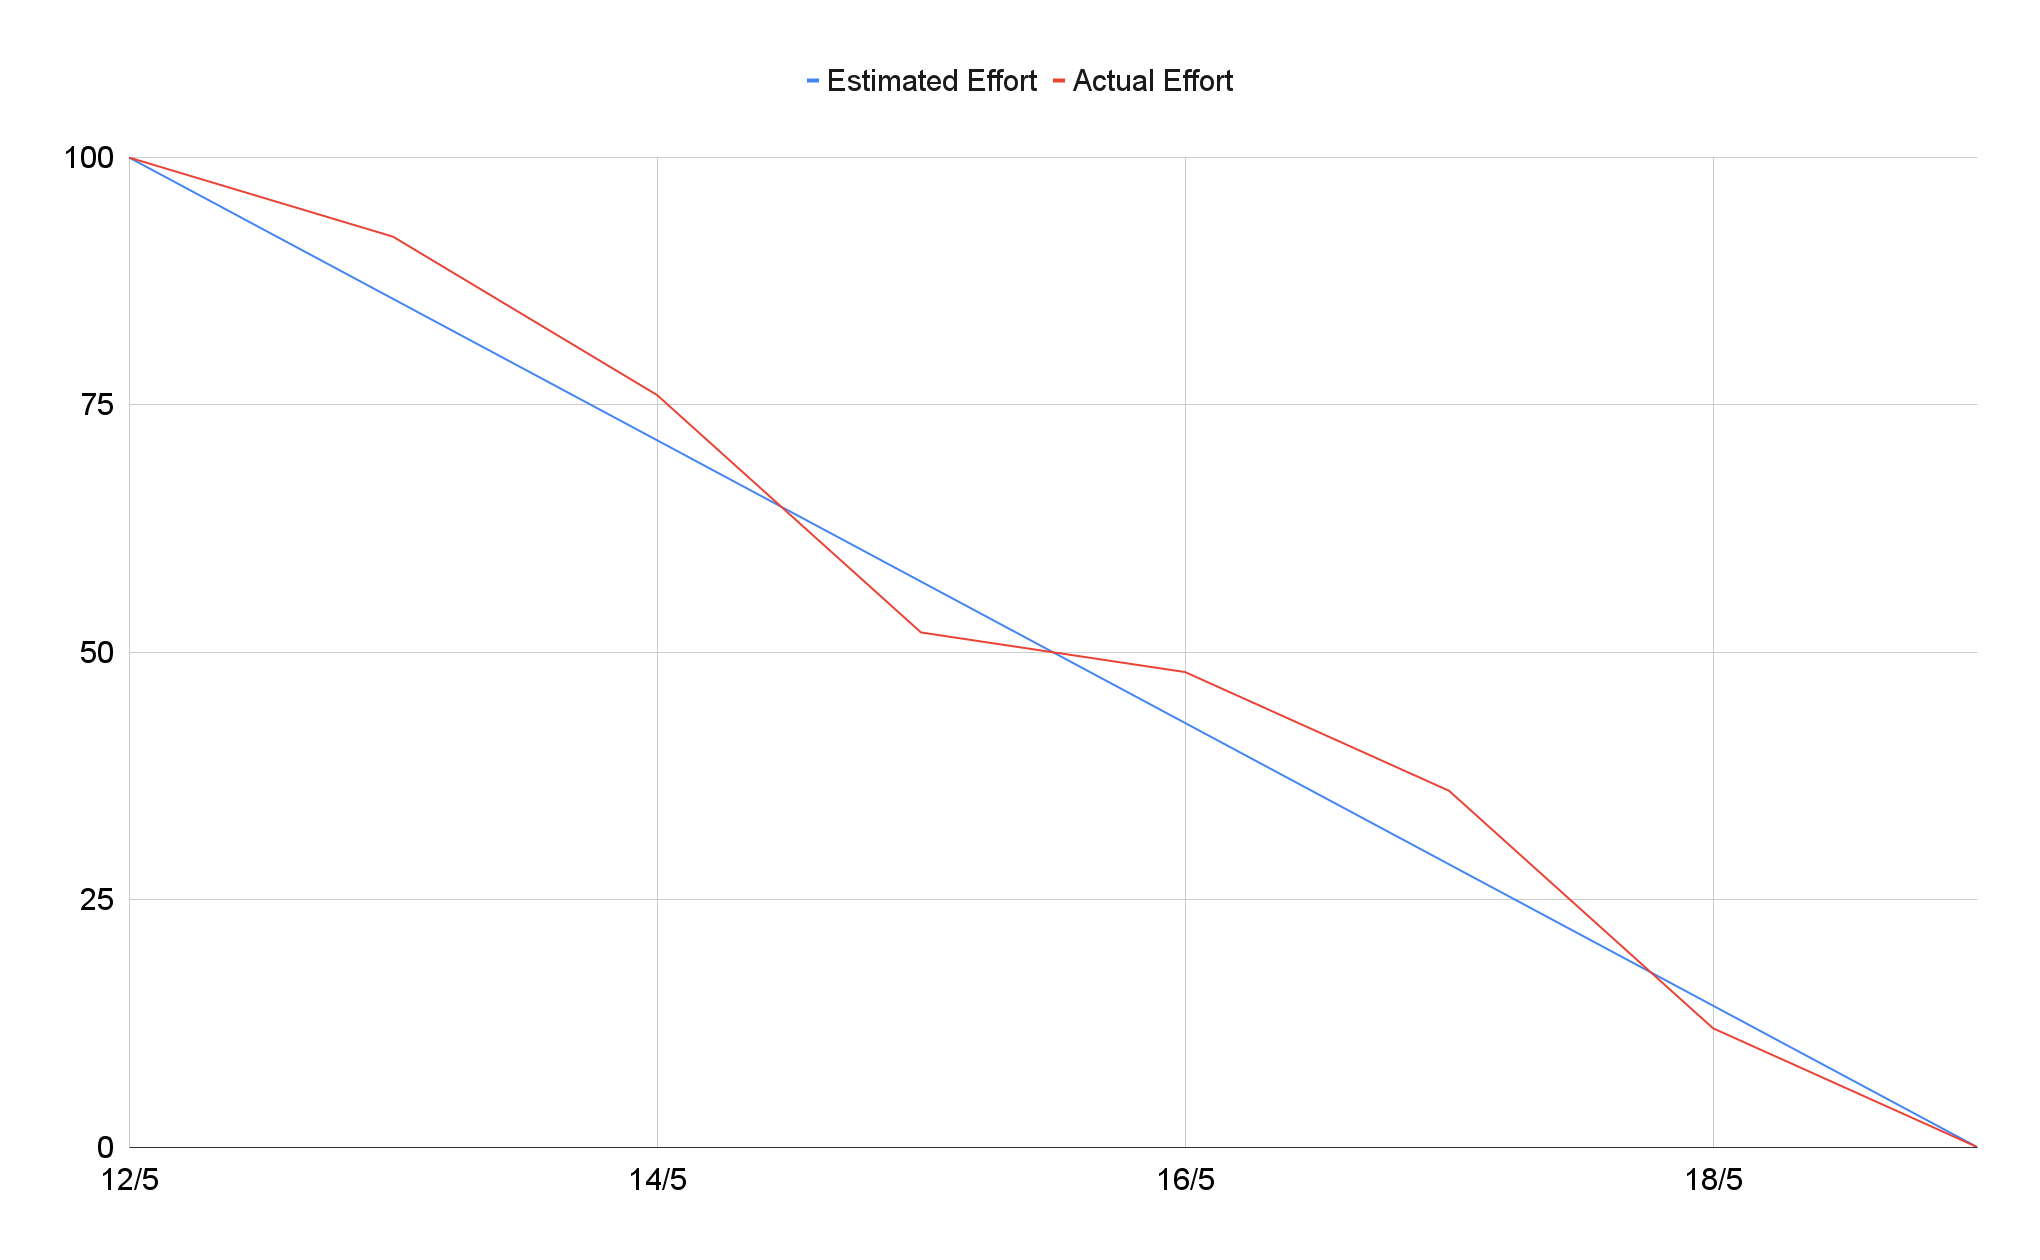
\includegraphics[width=0.95\textwidth]{images/burndown_chart.png}

\end{document}
